\documentclass[12pt, a4paper]{article}

\usepackage[margin=2.5cm]{geometry}
\usepackage{titling}   
\usepackage[english]{babel}
\usepackage{algorithm}
\usepackage[noend]{algpseudocode}
\usepackage{amsmath,amsthm,amssymb}
\usepackage{fancyhdr} 
\usepackage{xcolor}
\usepackage{colortbl}
\usepackage{minted}
\usepackage{hyperref}
\usepackage{graphicx}
\usepackage{enumitem}
\usepackage{xeCJK}
\usepackage{listings}
\usepackage[utf8]{inputenc}
\setCJKmainfont{Noto Serif CJK TC}
\definecolor{lightgray}{rgb}{0.95,0.95,0.95}

\lstset{
    backgroundcolor=\color{lightgray},
    basicstyle=\ttfamily\small,
    keywordstyle=\color{black},
    commentstyle=\color{blue},
    stringstyle=\color{red},
    showstringspaces=false,
    breaklines=true,
    numberstyle=\tiny\color{gray},
    escapeinside=||,
}

\algrenewcommand\algorithmicfunction{}
\pagestyle{fancy}
\fancyhf{}
\rhead{ROS2 Homework \#1}
\lhead{\fontsize{11}{15}\selectfont Formula SAE Training}
\cfoot{\thepage}

\title{\textbf{ROS2 Homework \#1}}

\author{李馥安 \\ CSIE B13902019}

\date{\today}

\begin{document}
\tableofcontents

\setcounter{section}{-1}
\maketitle
\section{Setup}
Since I am using Arch Linux, I modified the \texttt{install.sh} script accordingly. On Arch Linux, Python packages are named with the prefix \texttt{python-} and, once installed, they are available for the system's Python 3 intepreter.
\begin{lstlisting}[language=bash]
...
# install python modules
sudo pacman -Sy python-argcomplete \
		python-docker \
		python-prettytable \
		python-yaml
...
\end{lstlisting}
Activate shell completion:
\begin{lstlisting}[language=bash]
activate-global-python-argcomplete
source /etc/bash_completion.d/python-argcomplete
\end{lstlisting}
Build needed image:
\begin{lstlisting}[language=bash]
nturt_docker image build nturacing/nturt_ros:host-devel
\end{lstlisting}
Create a new container:
\begin{lstlisting}[language=bash]
nturt_docker container create 0731 nturacing/nturt_ros:host-devel host
\end{lstlisting}
Attach shell into container:
\begin{lstlisting}[language=bash]
nturt_docker container shell 0731
\end{lstlisting}

\newpage
\section{Beginner: CLI tools}
\subsection{Configuring environment}
Most of the environment configuration is done automatically when starting the Docker container. However, it is important to note that the \texttt{ROS\_DISTRO} is set to \texttt{iron}, so when installing packages, I need to make sure to use the package repositories corresponding to the Iron distribution instead of Humble distribution.


\subsection{Using \texttt{turtlesim, ros2} and \texttt{rqt}}
\begin{enumerate}
	\item Install \texttt{turtlesim}\\
		I found the password for root and user "docker" is \texttt{docker} in \\\texttt{Dockerfile/nturt\_ros/host/devel/Dockerfile }.
\begin{lstlisting}[language=bash]
sudo apt update
sudo apt install ros-iron-turtlesim
\end{lstlisting}
And I found that it has been installed already in the container.\\
\begin{figure}[h]
	\setlength{\leftskip}{2.4em}
	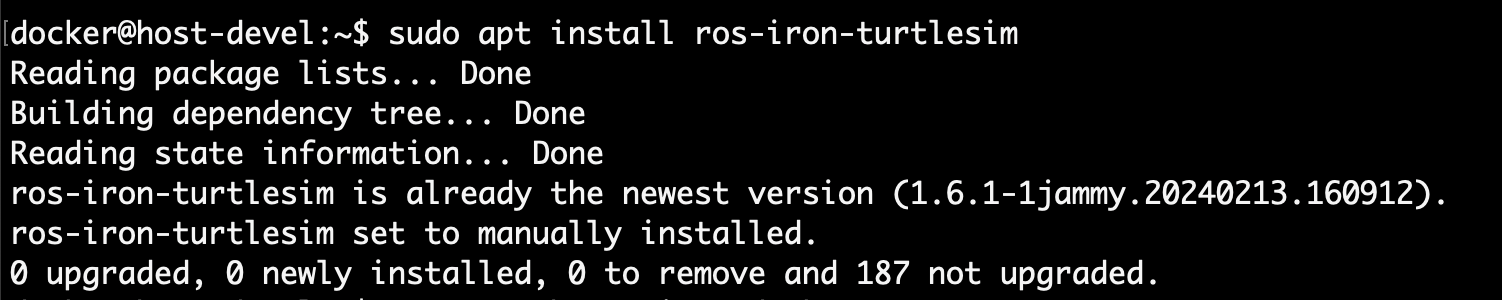
\includegraphics[width=0.94\textwidth]{p1.2-1}
\end{figure}

Double check whether the package is installed:
\begin{lstlisting}[language=bash]
ros2 pkg executables turtlesim
\end{lstlisting}
\begin{figure}[h]
	\setlength{\leftskip}{2.4em}
	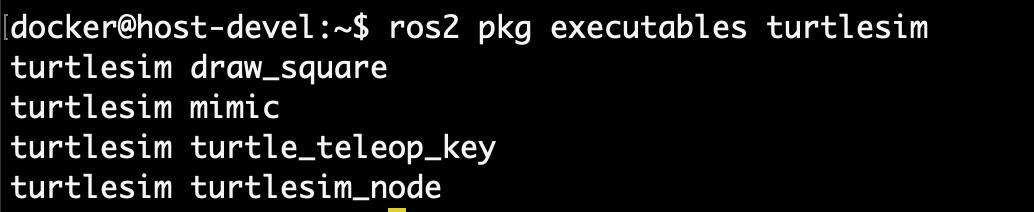
\includegraphics[width=0.94\textwidth]{p1.2-2}
\end{figure}
\item Start turtlesim
\begin{lstlisting}[language=bash]
ros2 run turtlesim turtlesim_node
\end{lstlisting}
\begin{figure}[h]
	\setlength{\leftskip}{2.4em}
	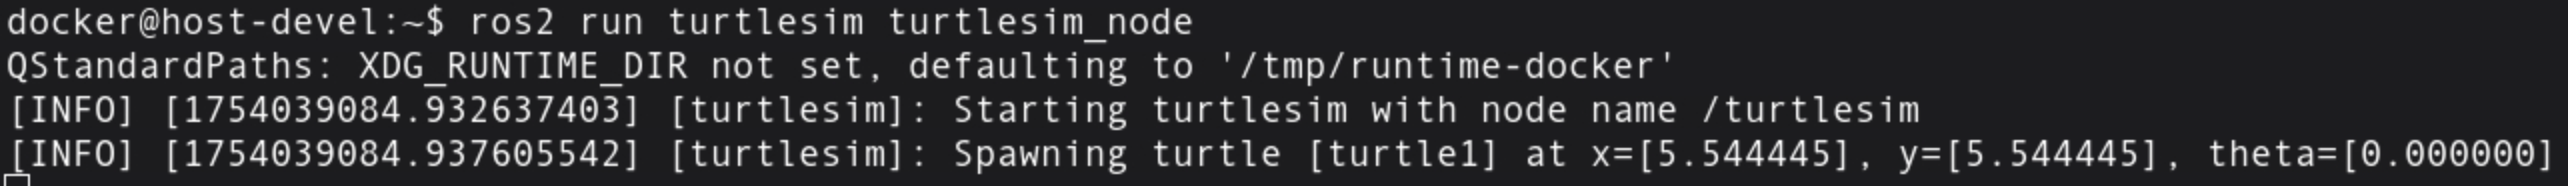
\includegraphics[width=0.94\textwidth]{p1.2-3}
\end{figure}
\newpage
\item Use turtlesim
\begin{lstlisting}[language=bash]
ros2 run turtlesim turtle_teleop_key
\end{lstlisting}
\begin{figure}[h]
	\setlength{\leftskip}{2.4em}
	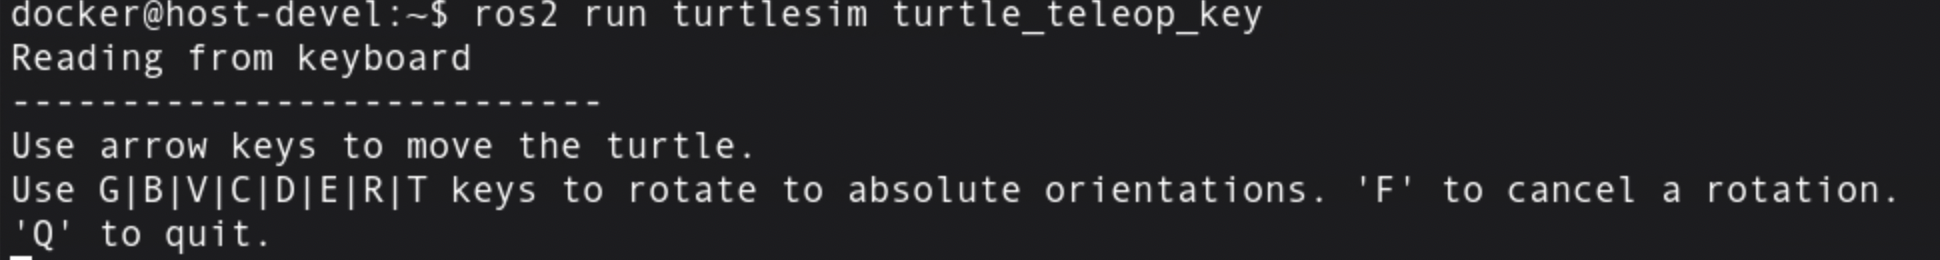
\includegraphics[width=0.94\textwidth]{p1.2-4}
\end{figure}
\begin{figure}[h]
	\centering
	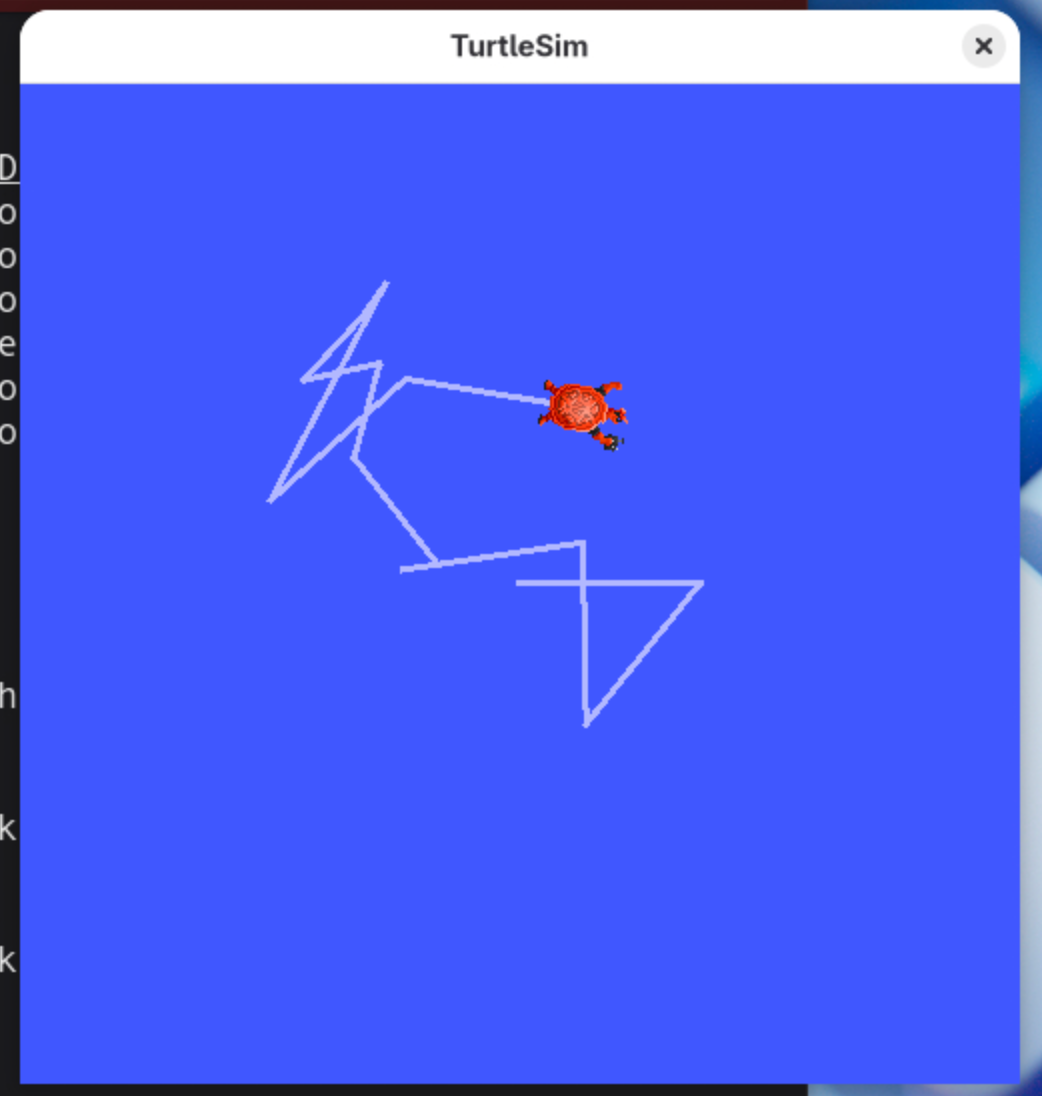
\includegraphics[width=0.5\textwidth]{p1.2-5}
\end{figure}
By using the \texttt{list} subcommands, I can see the nodes, topics, services, and actions.
\begin{lstlisting}[language=bash]
ros2 node list
ros2 topic list
ros2 service list
ros2 action list
\end{lstlisting}
\begin{figure}[h]
	\centering
	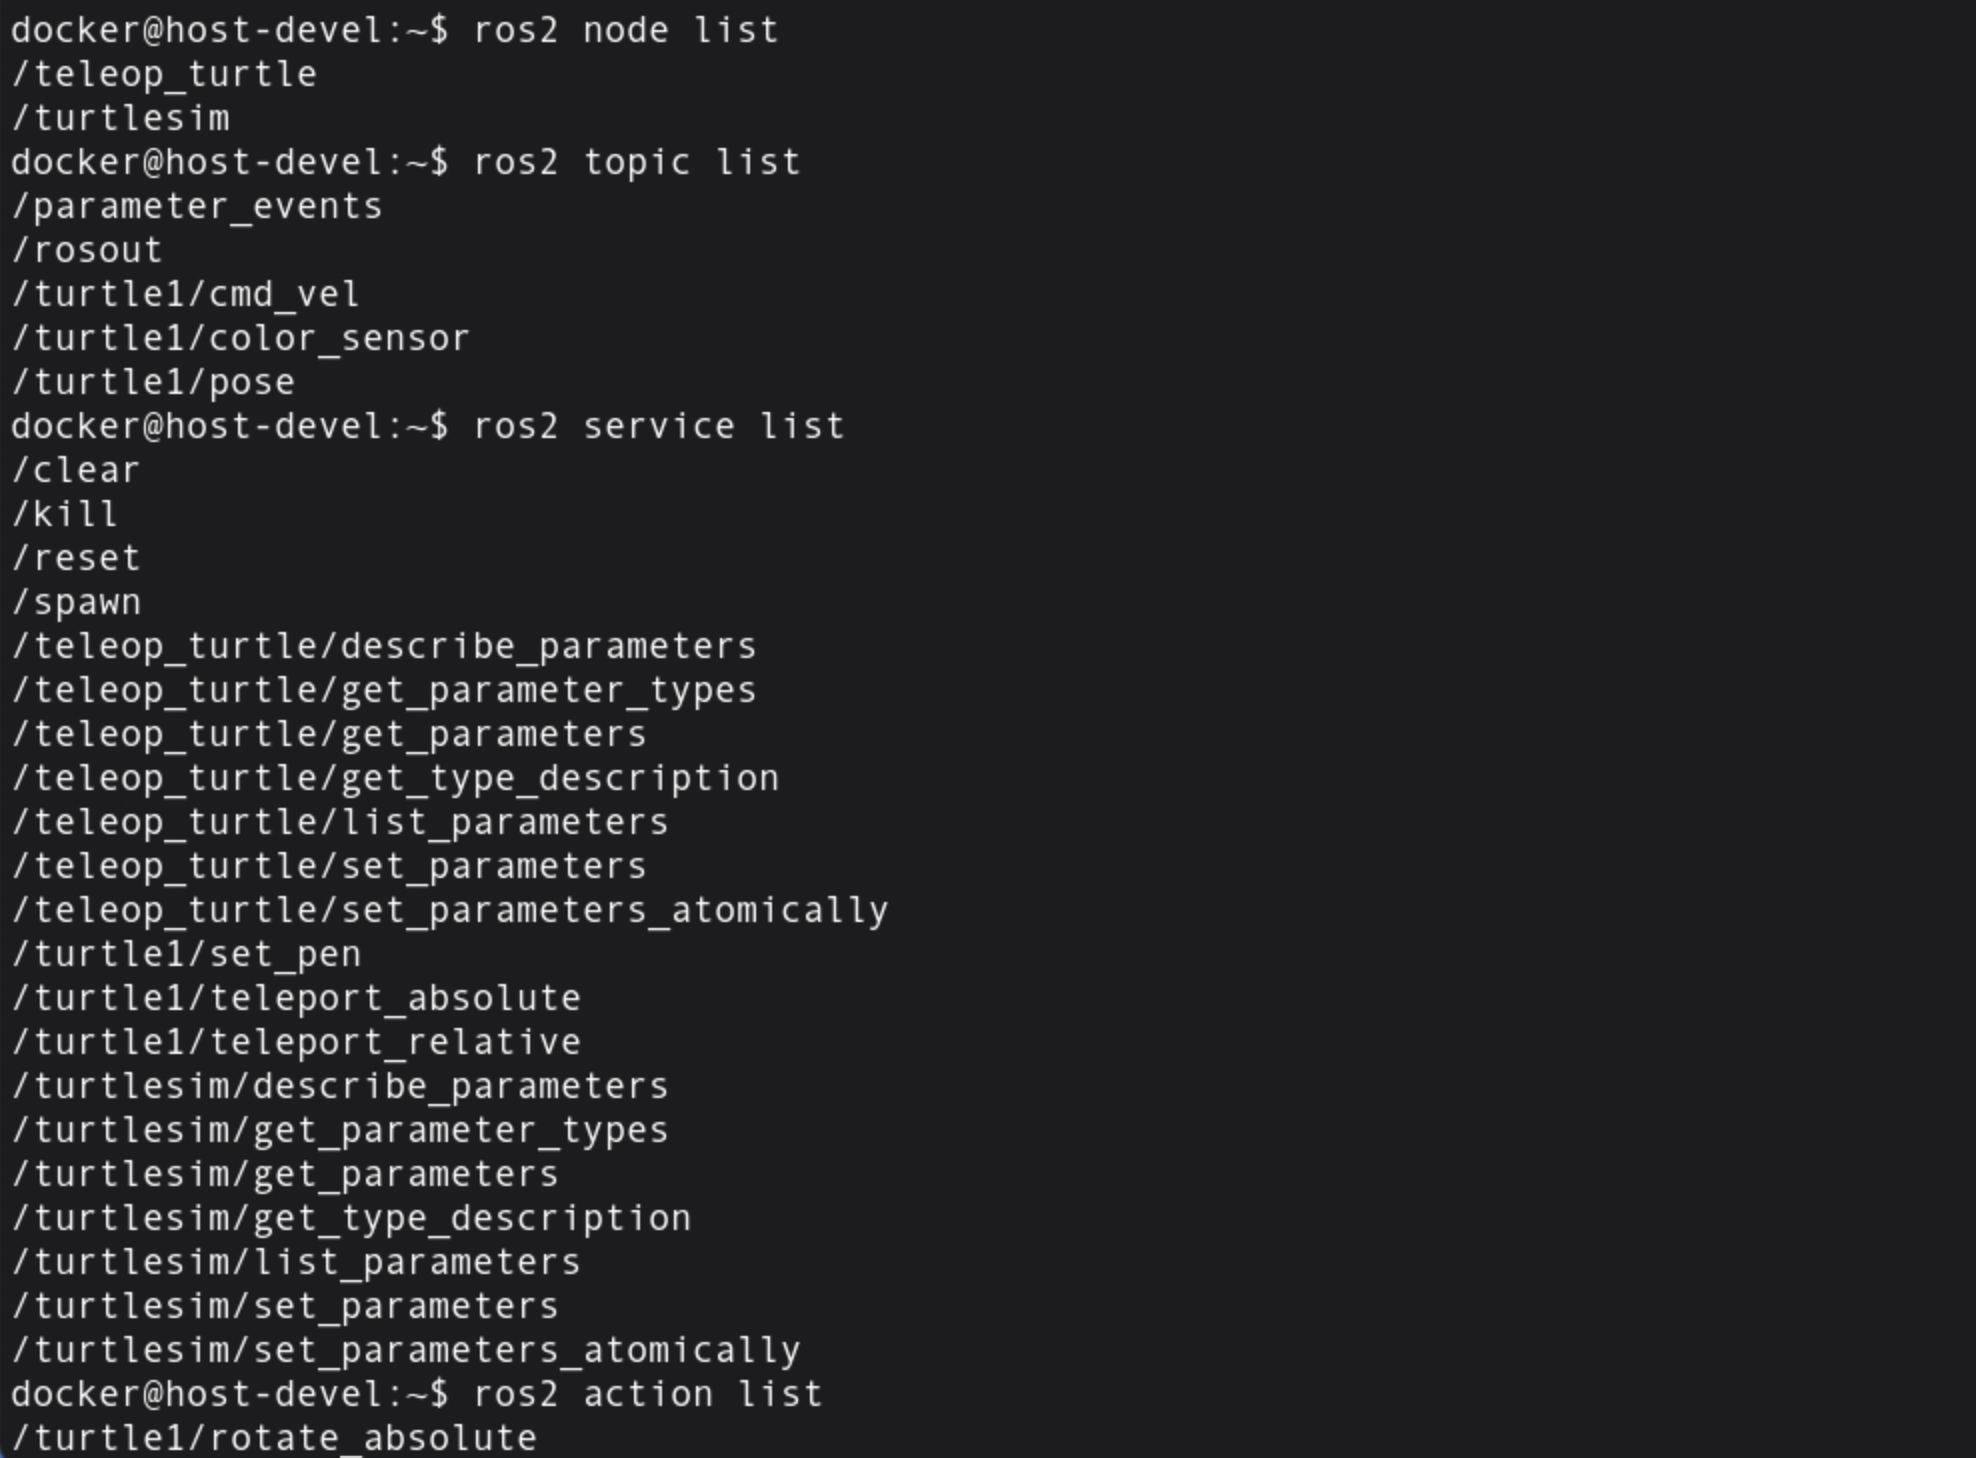
\includegraphics[width=0.9\textwidth]{p1.2-6}
\end{figure}
\newpage
\item Install rqt\\
	Similarly, after checking, the \texttt{ros2-iron-rqt} packages has been installed in the container.\\
	Run \texttt{rqt}:
\begin{lstlisting}[language=bash]
rqt
\end{lstlisting}
\begin{figure}[h]
	\setlength{\leftskip}{2.4em}
	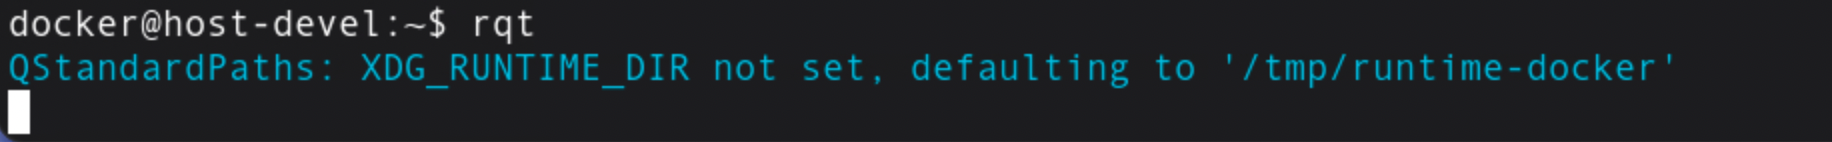
\includegraphics[width=0.94\textwidth]{p1.2-7}
\end{figure}
\begin{figure}[h]
	\centering
	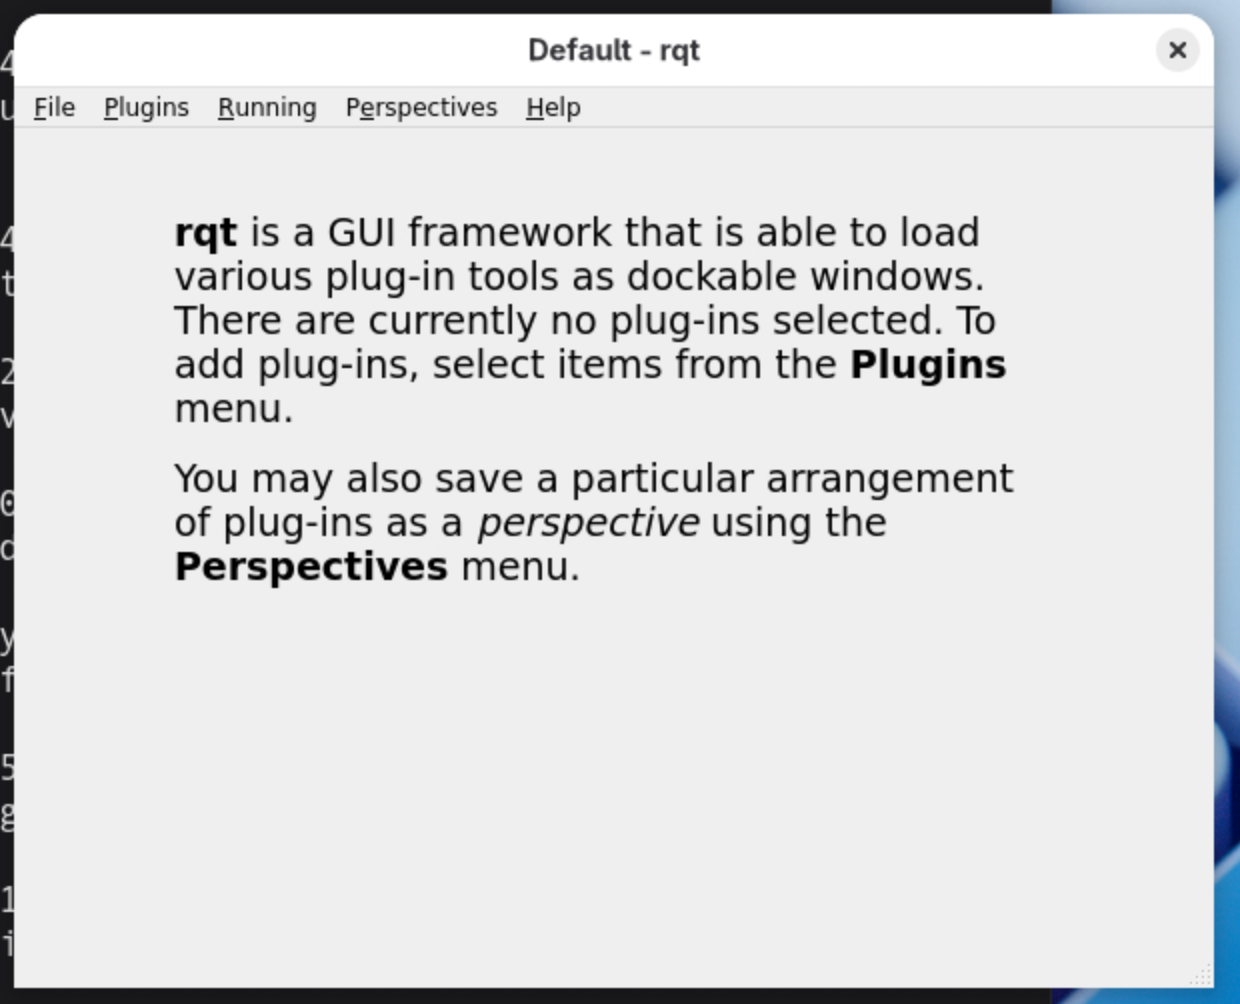
\includegraphics[width=0.4\textwidth]{p1.2-8}
\end{figure}
\newpage
\item Use rqt\\
	Select \texttt{Plugins} > \texttt{Services} > \texttt{Service Caller}:
\begin{figure}[h]
	\centering
	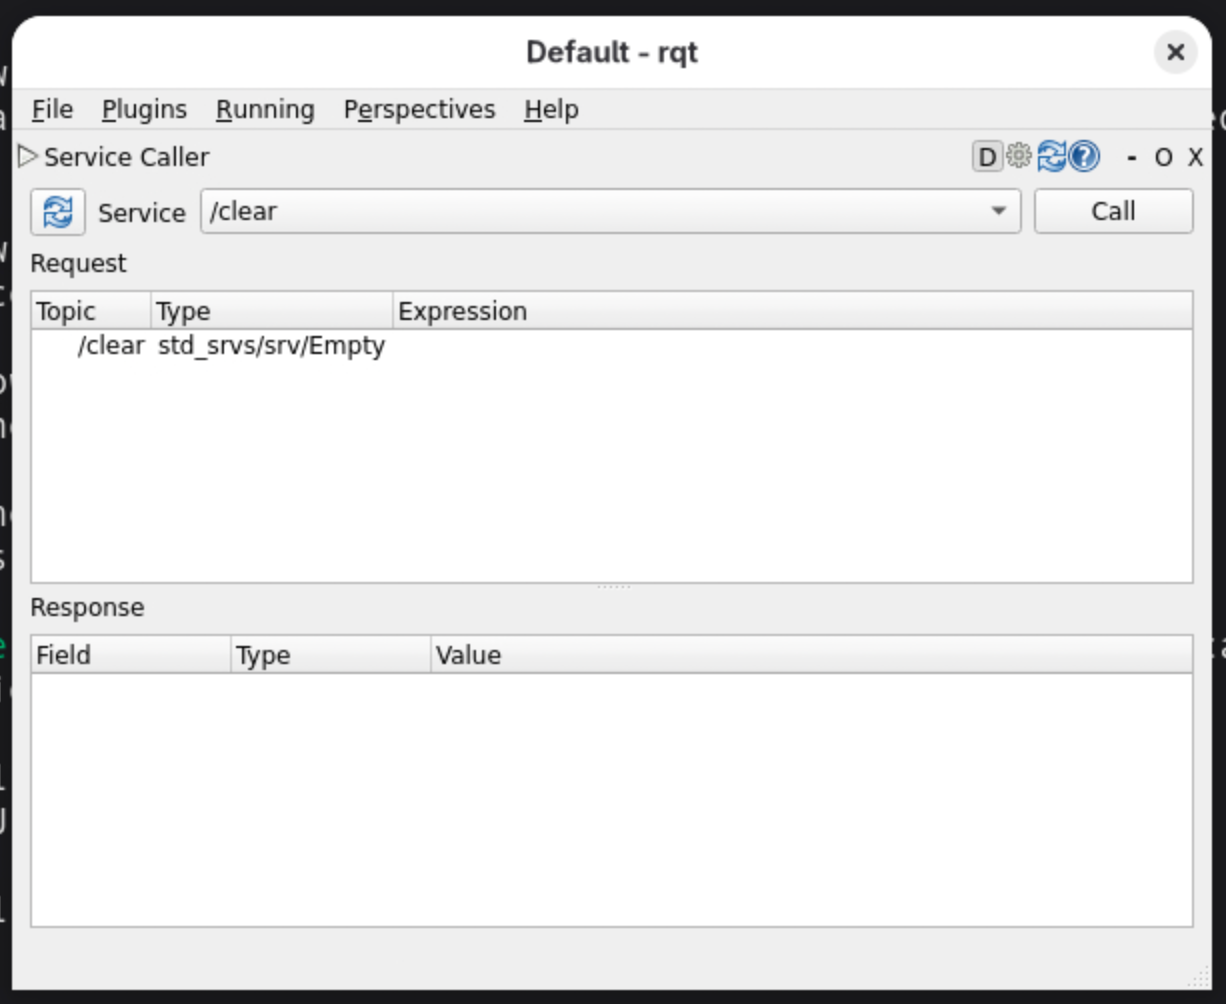
\includegraphics[width=0.4\textwidth]{p1.2-9}
\end{figure}
\begin{enumerate}
	\item Try the spawn service
\begin{figure}[h]
	\centering
	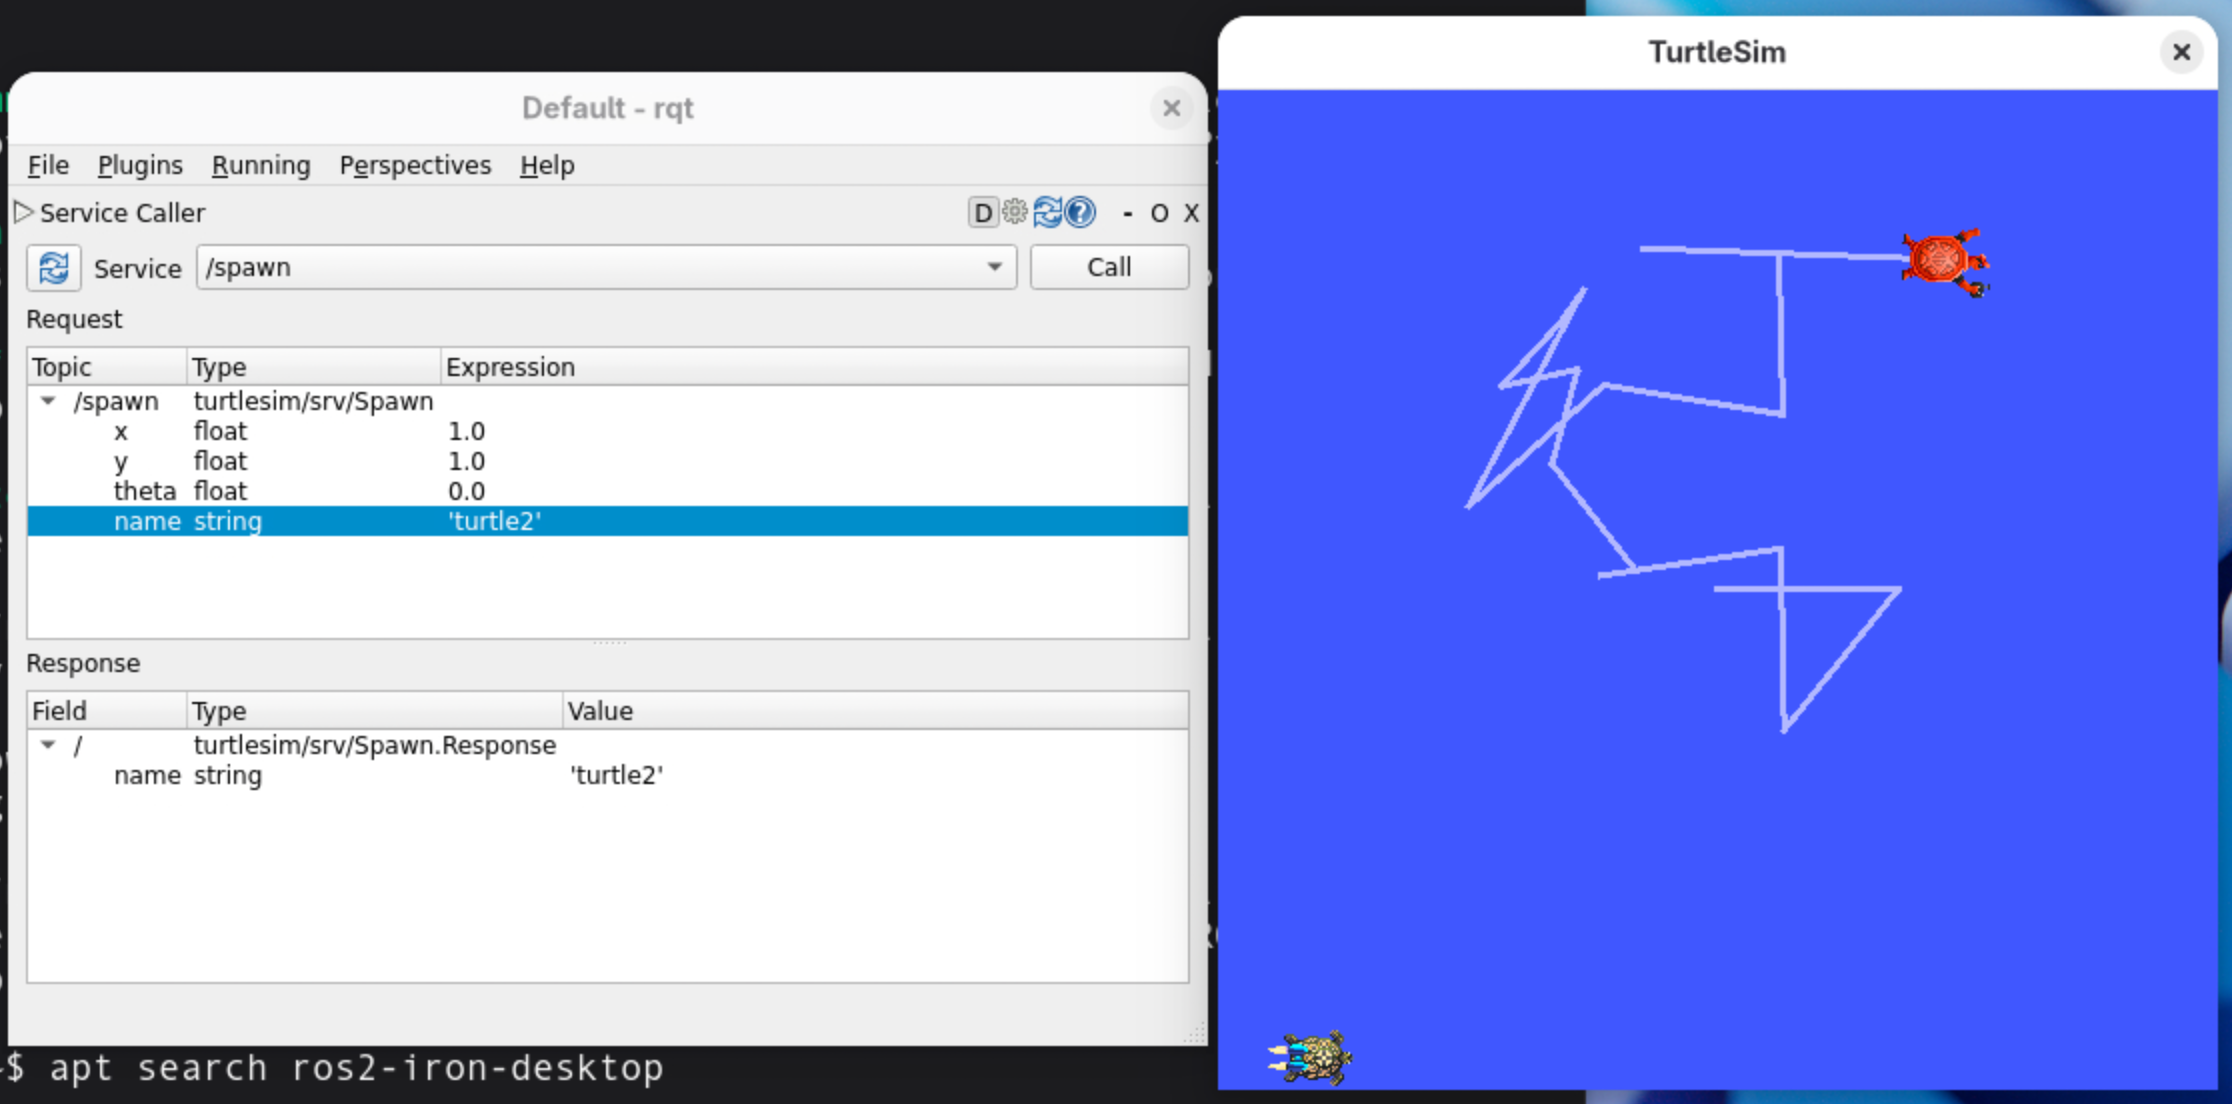
\includegraphics[width=0.7\textwidth]{p1.2-10}
\end{figure}
	\item Try the set\_pen service
\begin{figure}[h]
	\centering
	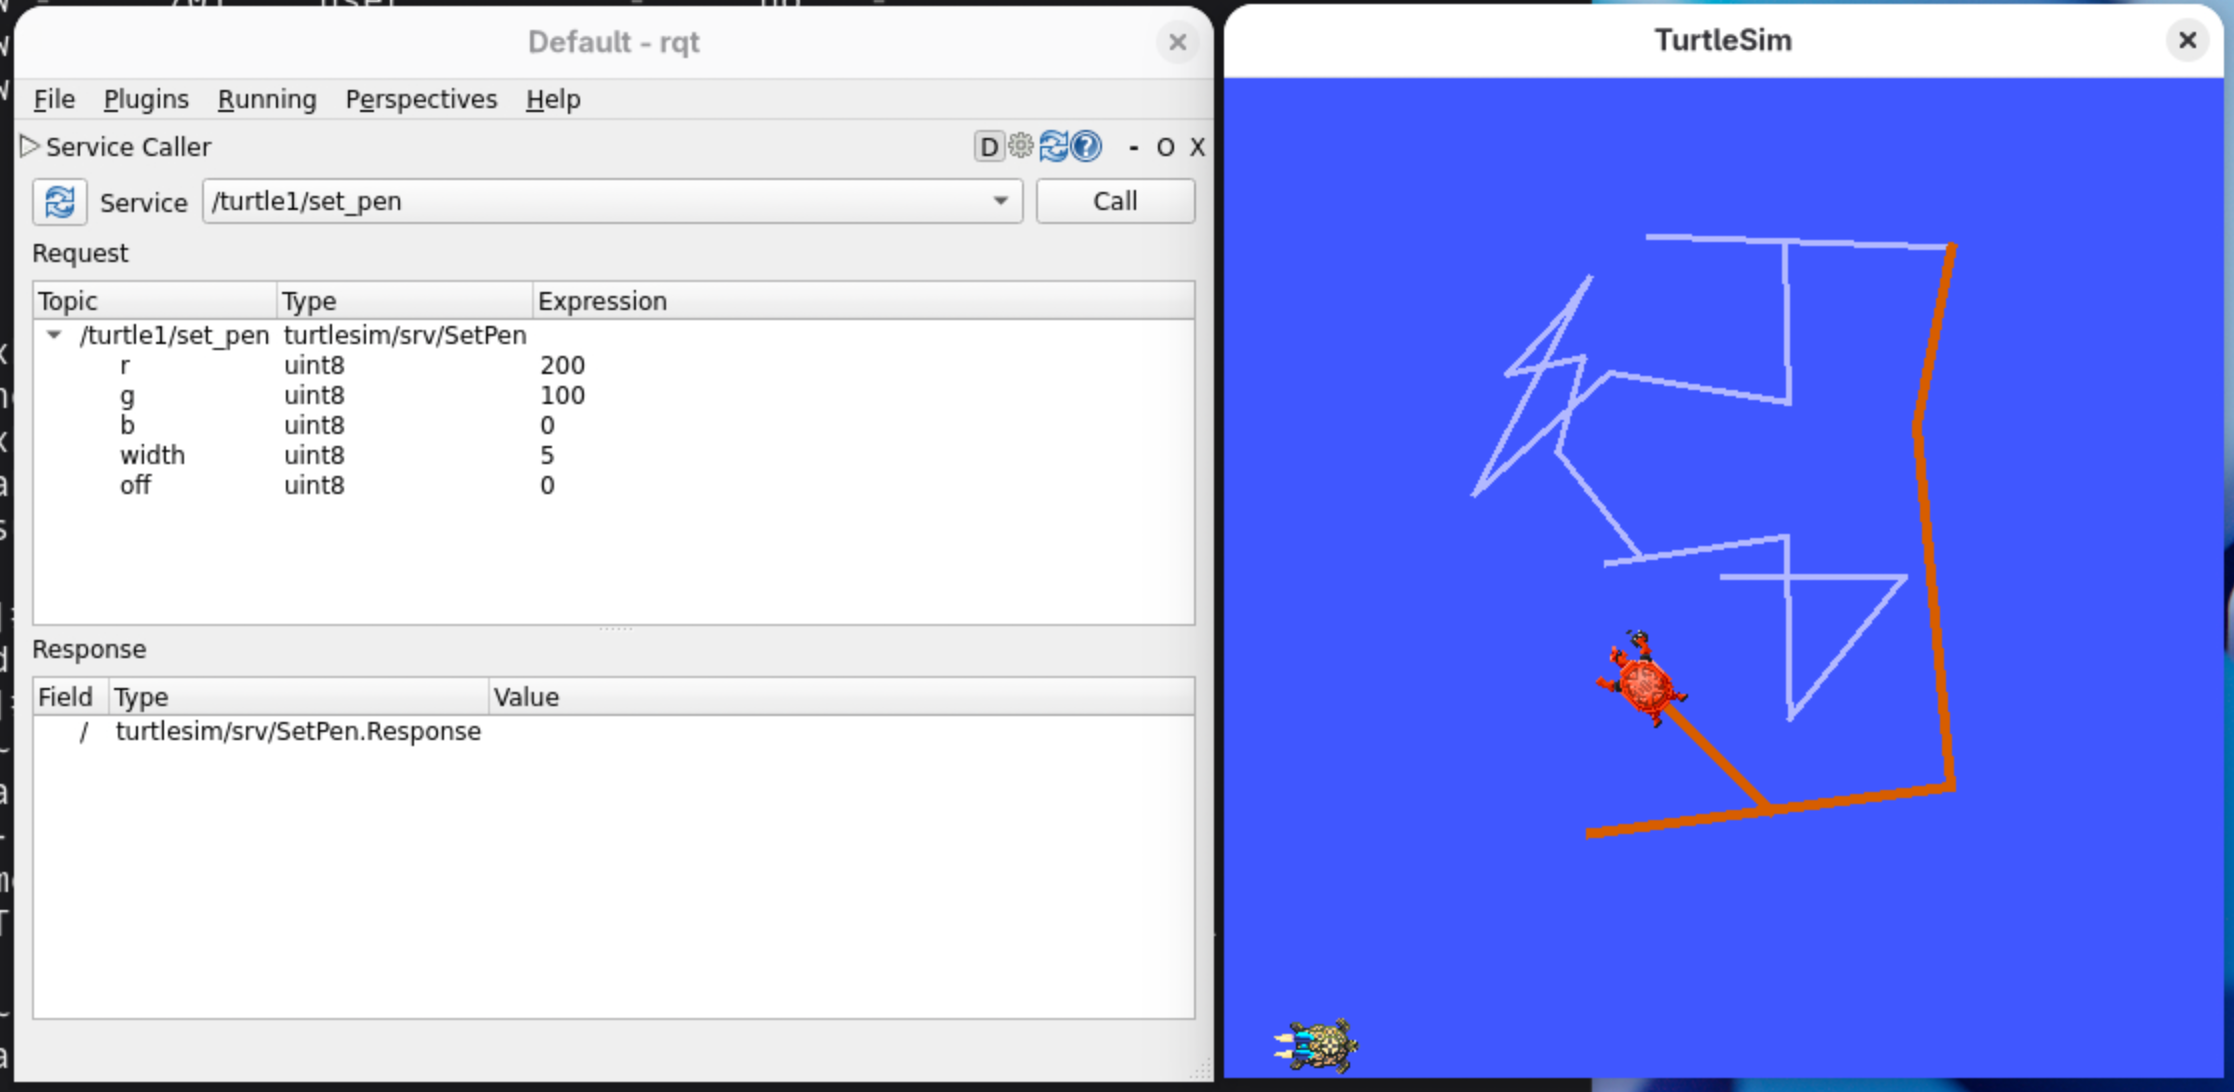
\includegraphics[width=0.7\textwidth]{p1.2-11}
\end{figure}

\end{enumerate}
\newpage
\item Remapping\\
	In order to control \texttt{turtle2}, I can't use the same command before, because it wil also contorl \texttt{turtle1} too. Instead, use the new command to remap the topic \texttt{cmd\_vel}:
\begin{lstlisting}[language=bash]
ros2 run turtlesim turtle_teleop_key --ros-args --remap turtle1/cmd_vel:=turtle2/cmd_vel
\end{lstlisting}
\begin{figure}[h]
	\setlength{\leftskip}{2.4em}
	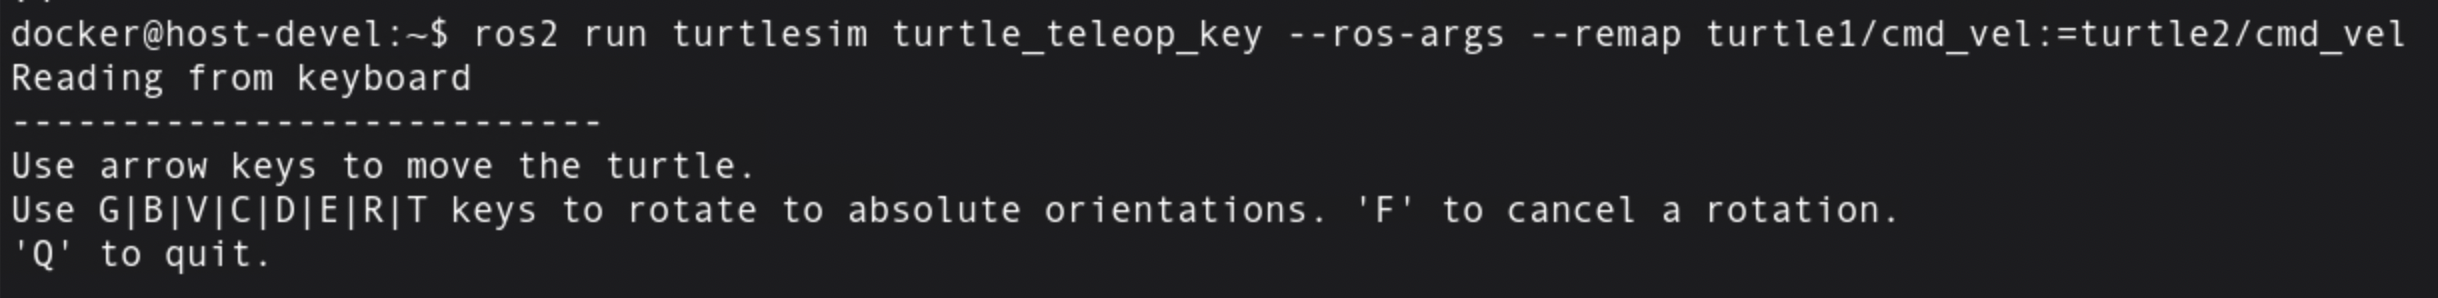
\includegraphics[width=0.94\textwidth]{p1.2-12}
\end{figure}
\begin{figure}[h]
	\centering
	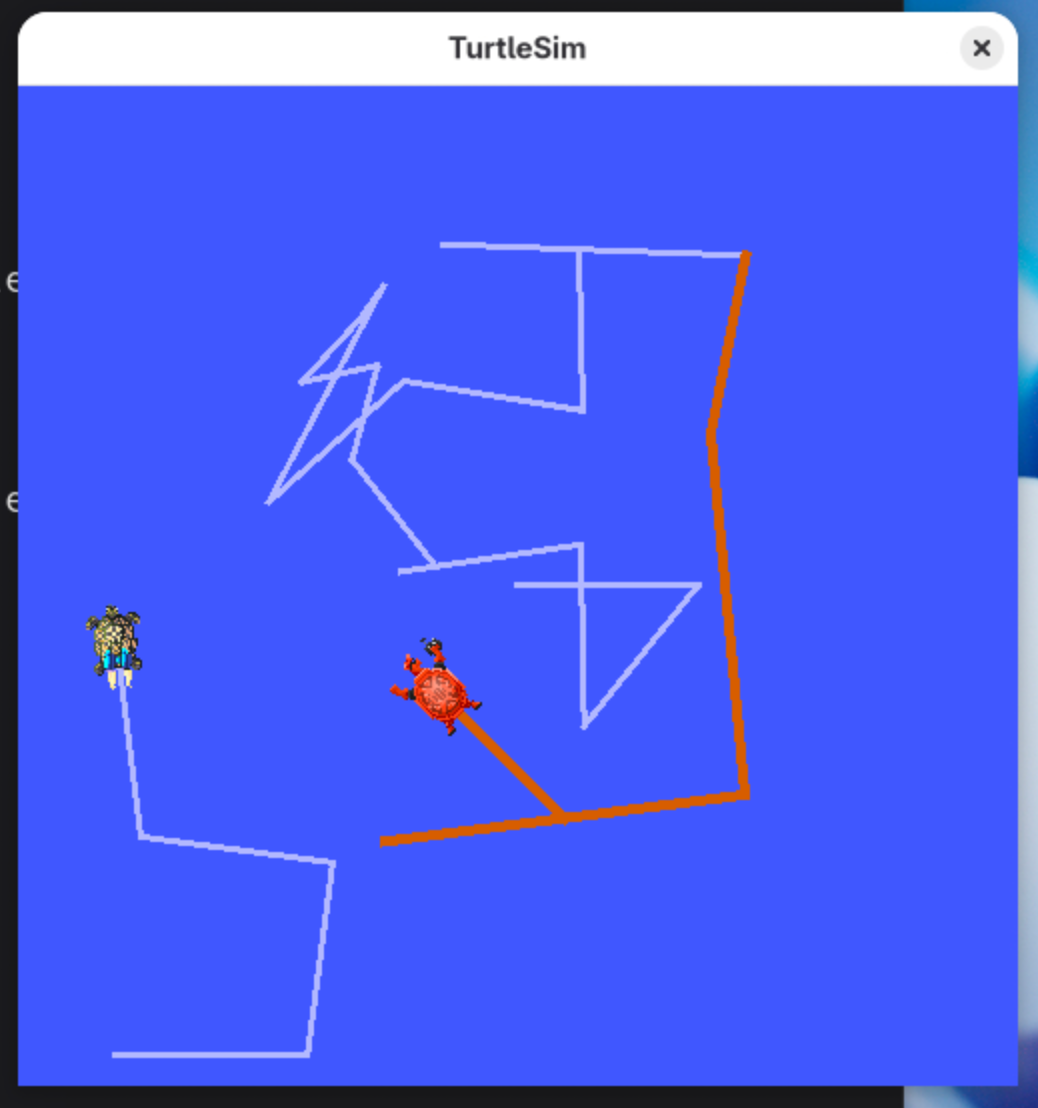
\includegraphics[width=0.4\textwidth]{p1.2-13}
\end{figure}
\item Close turtlesim\\
	Use \texttt{Ctrl+C} and \texttt{q} to close the terminals.
\end{enumerate}
\newpage
\subsection{Understanding nodes}
\begin{enumerate}
	\item ros2 run\\
		To launch an executable from a package:
\begin{lstlisting}[language=bash]
ros2 run <package> <executable>
\end{lstlisting}
For instance:
\begin{lstlisting}[language=bash]
ros2 run turtlesim turtlesim_node
\end{lstlisting}
And I got same result as the previous section got.
	\item ros2 node list\\
Show the running nodes:
\begin{lstlisting}[language=bash]
ros2 node list
\end{lstlisting}
\begin{itemize}
	\item Remapping\\
		Allow me to reassign default node properties, e.g. node name(by using \texttt{\_\_node}):
\begin{lstlisting}[language=bash]
ros2 run turtlesim turtlesim_node --ros-args --remap __node:myturtle
\end{lstlisting}
There will be a new node:
\begin{figure}[h]
	\setlength{\leftskip}{4.4em}
	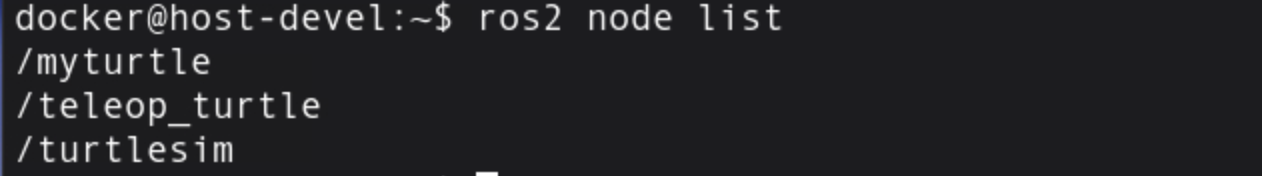
\includegraphics[width=0.88\textwidth]{p1.3-1}
\end{figure}
\end{itemize}
	\item ros2 node info
\begin{lstlisting}[language=bash]
ros2 node info /myturtle
\end{lstlisting}
\begin{figure}[h]
	\centering
	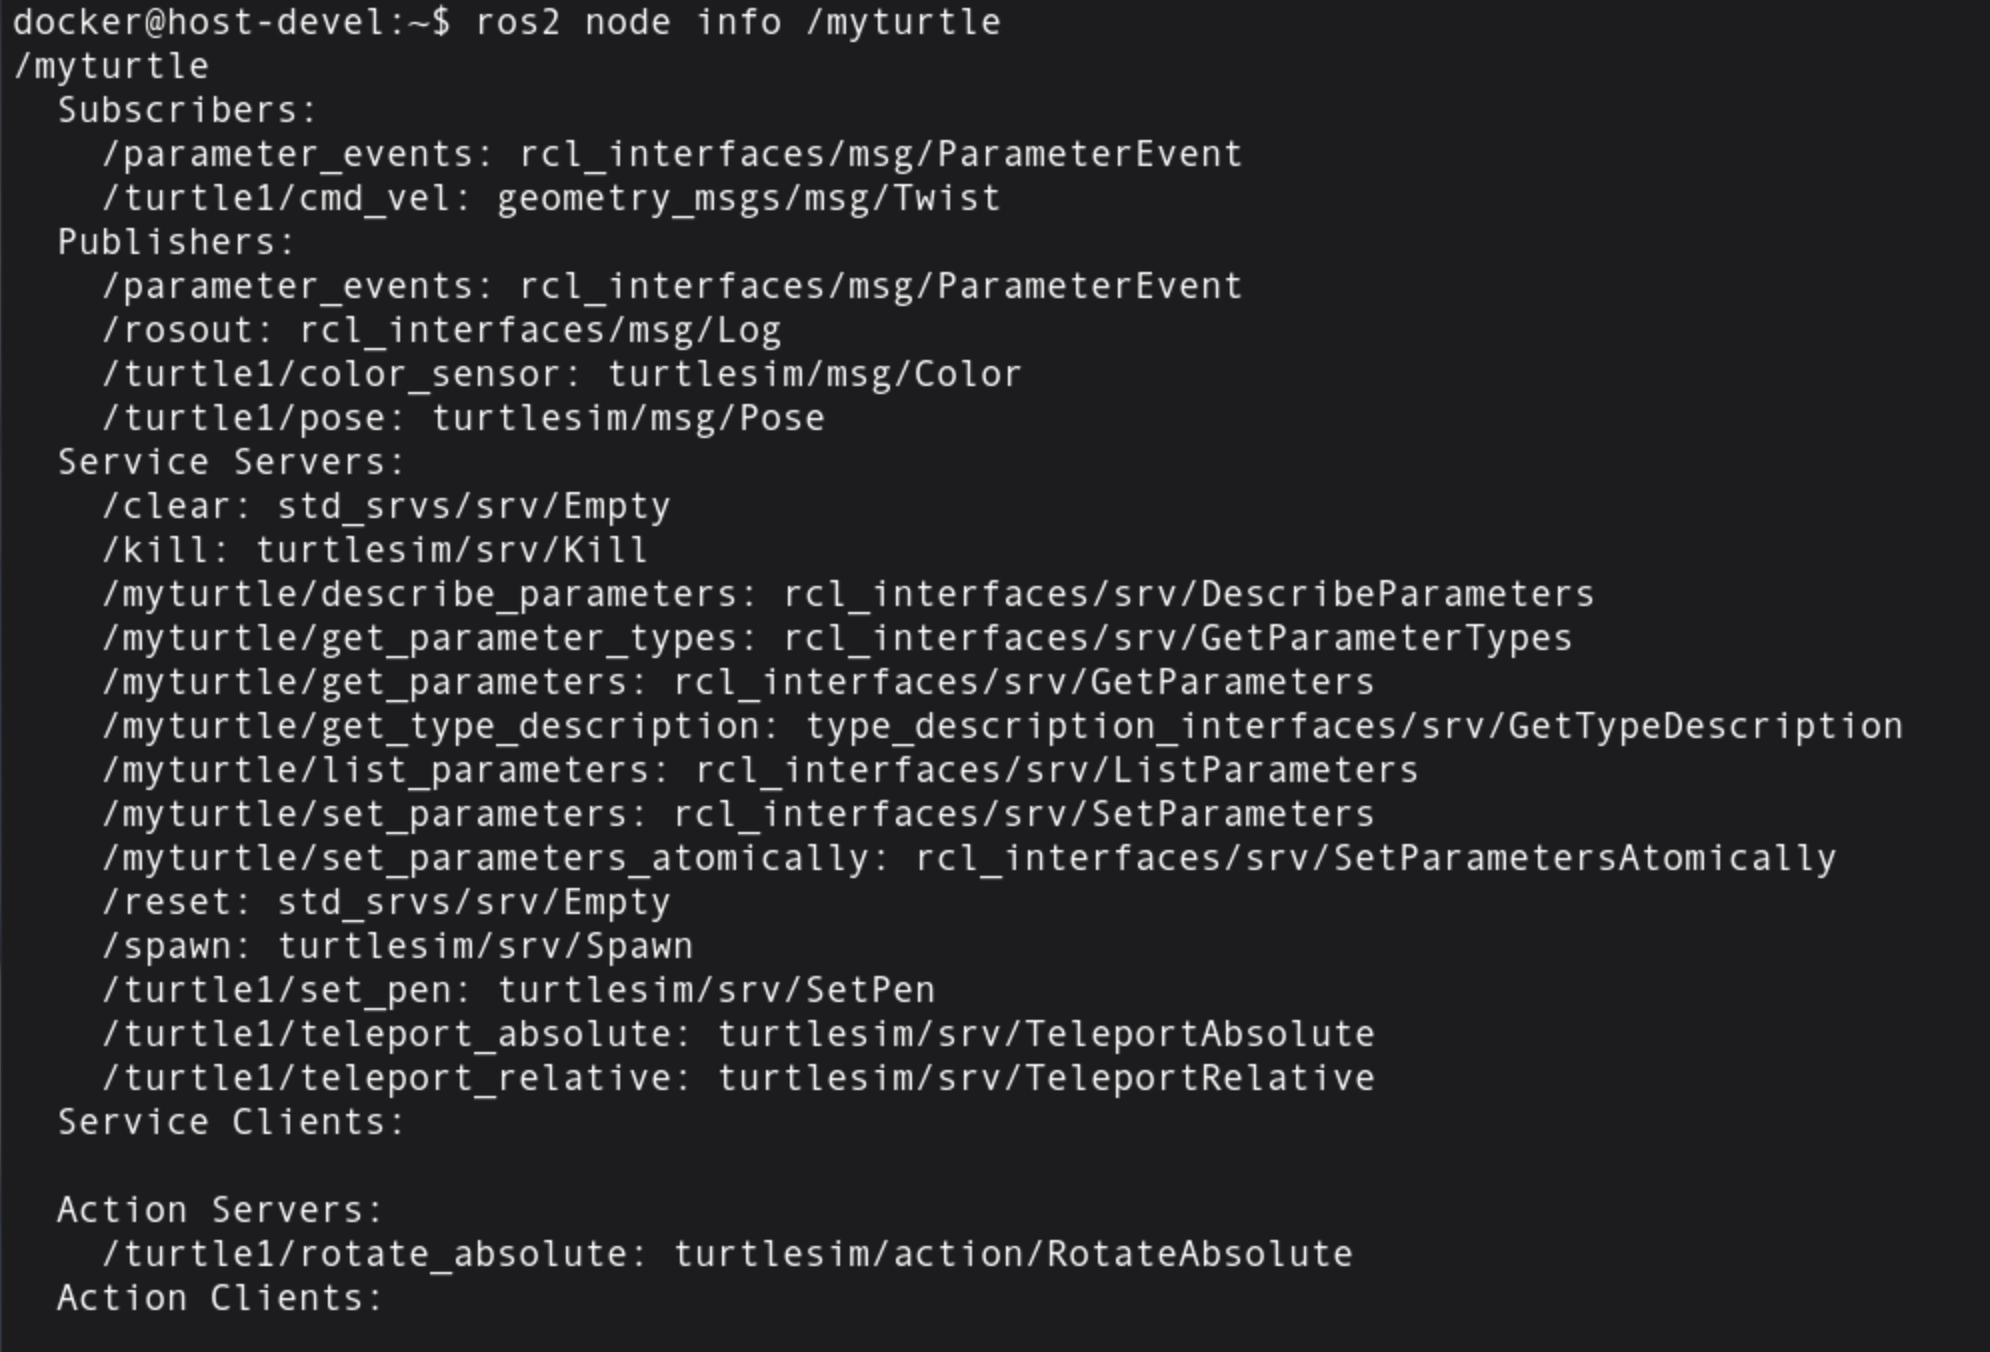
\includegraphics[width=0.74\textwidth]{p1.3-2}
\end{figure}
\end{enumerate}

\newpage
\subsection{Understanding topics}
\begin{enumerate}
	\item Setup
\begin{lstlisting}[language=bash]
ros2 run turtlesim turtlesim_node
ros2 run turtlesim turtlesim_teleop_key
\end{lstlisting}
	\item rqt\_graph
\begin{lstlisting}[language=bash]
rqt_graph
\end{lstlisting}
\begin{figure}[h]
	\centering
	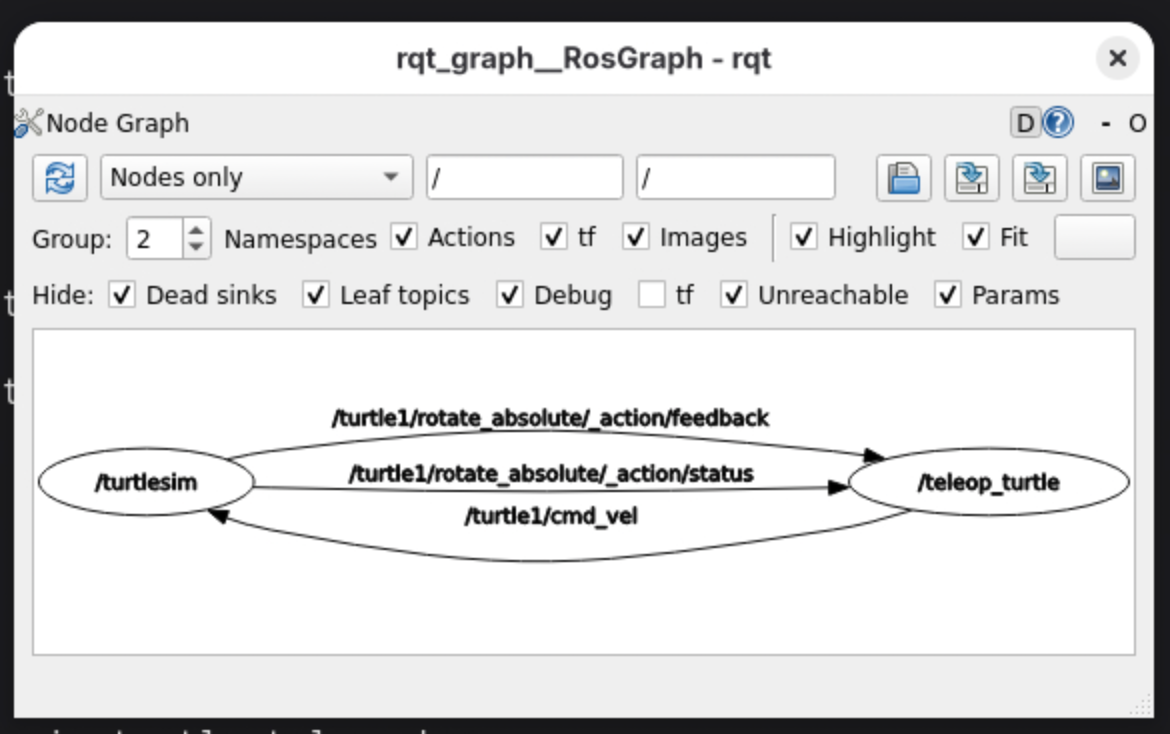
\includegraphics[width=0.6\textwidth]{p1.4-1}
\end{figure}
We can discover that \texttt{/teleop\_turtle} publishes data to the topic \texttt{/turtle1/cmd\_vel}, and \texttt{/turtlesim} is subscribed to it.
\item ros2 topic list
\begin{lstlisting}[language=bash]
ros2 ropic list
\end{lstlisting}
Return currently active topics:
\begin{figure}[h]
	\setlength{\leftskip}{2.4em}
	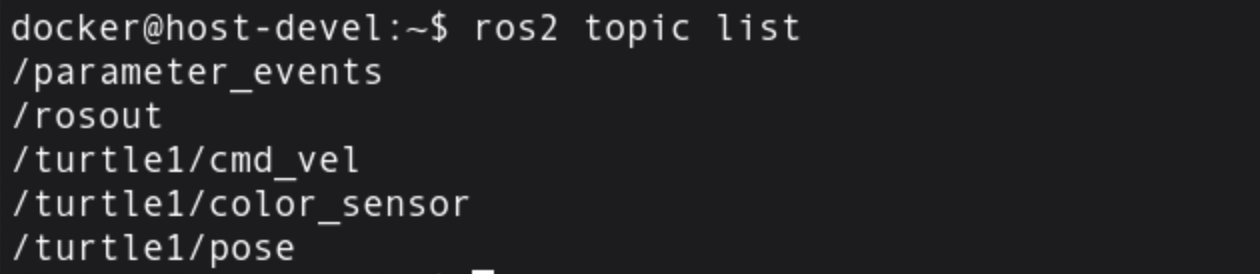
\includegraphics[width=0.94\textwidth]{p1.4-2}
\end{figure}
With the flag \texttt{-t}, I get more information of topic type appended in bracket.
\begin{lstlisting}[language=bash]
ros2 topic list -t
\end{lstlisting}
\begin{figure}[h]
	\setlength{\leftskip}{2.4em}
	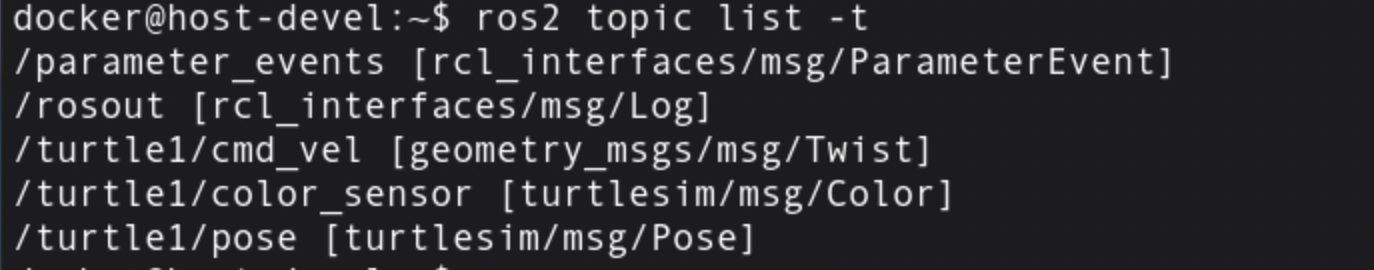
\includegraphics[width=0.94\textwidth]{p1.4-3}
\end{figure}
\newpage
Uncheck all boxes under Hider can see all topics on \texttt{rqt\_graph}:
\begin{figure}[h]
	\centering
	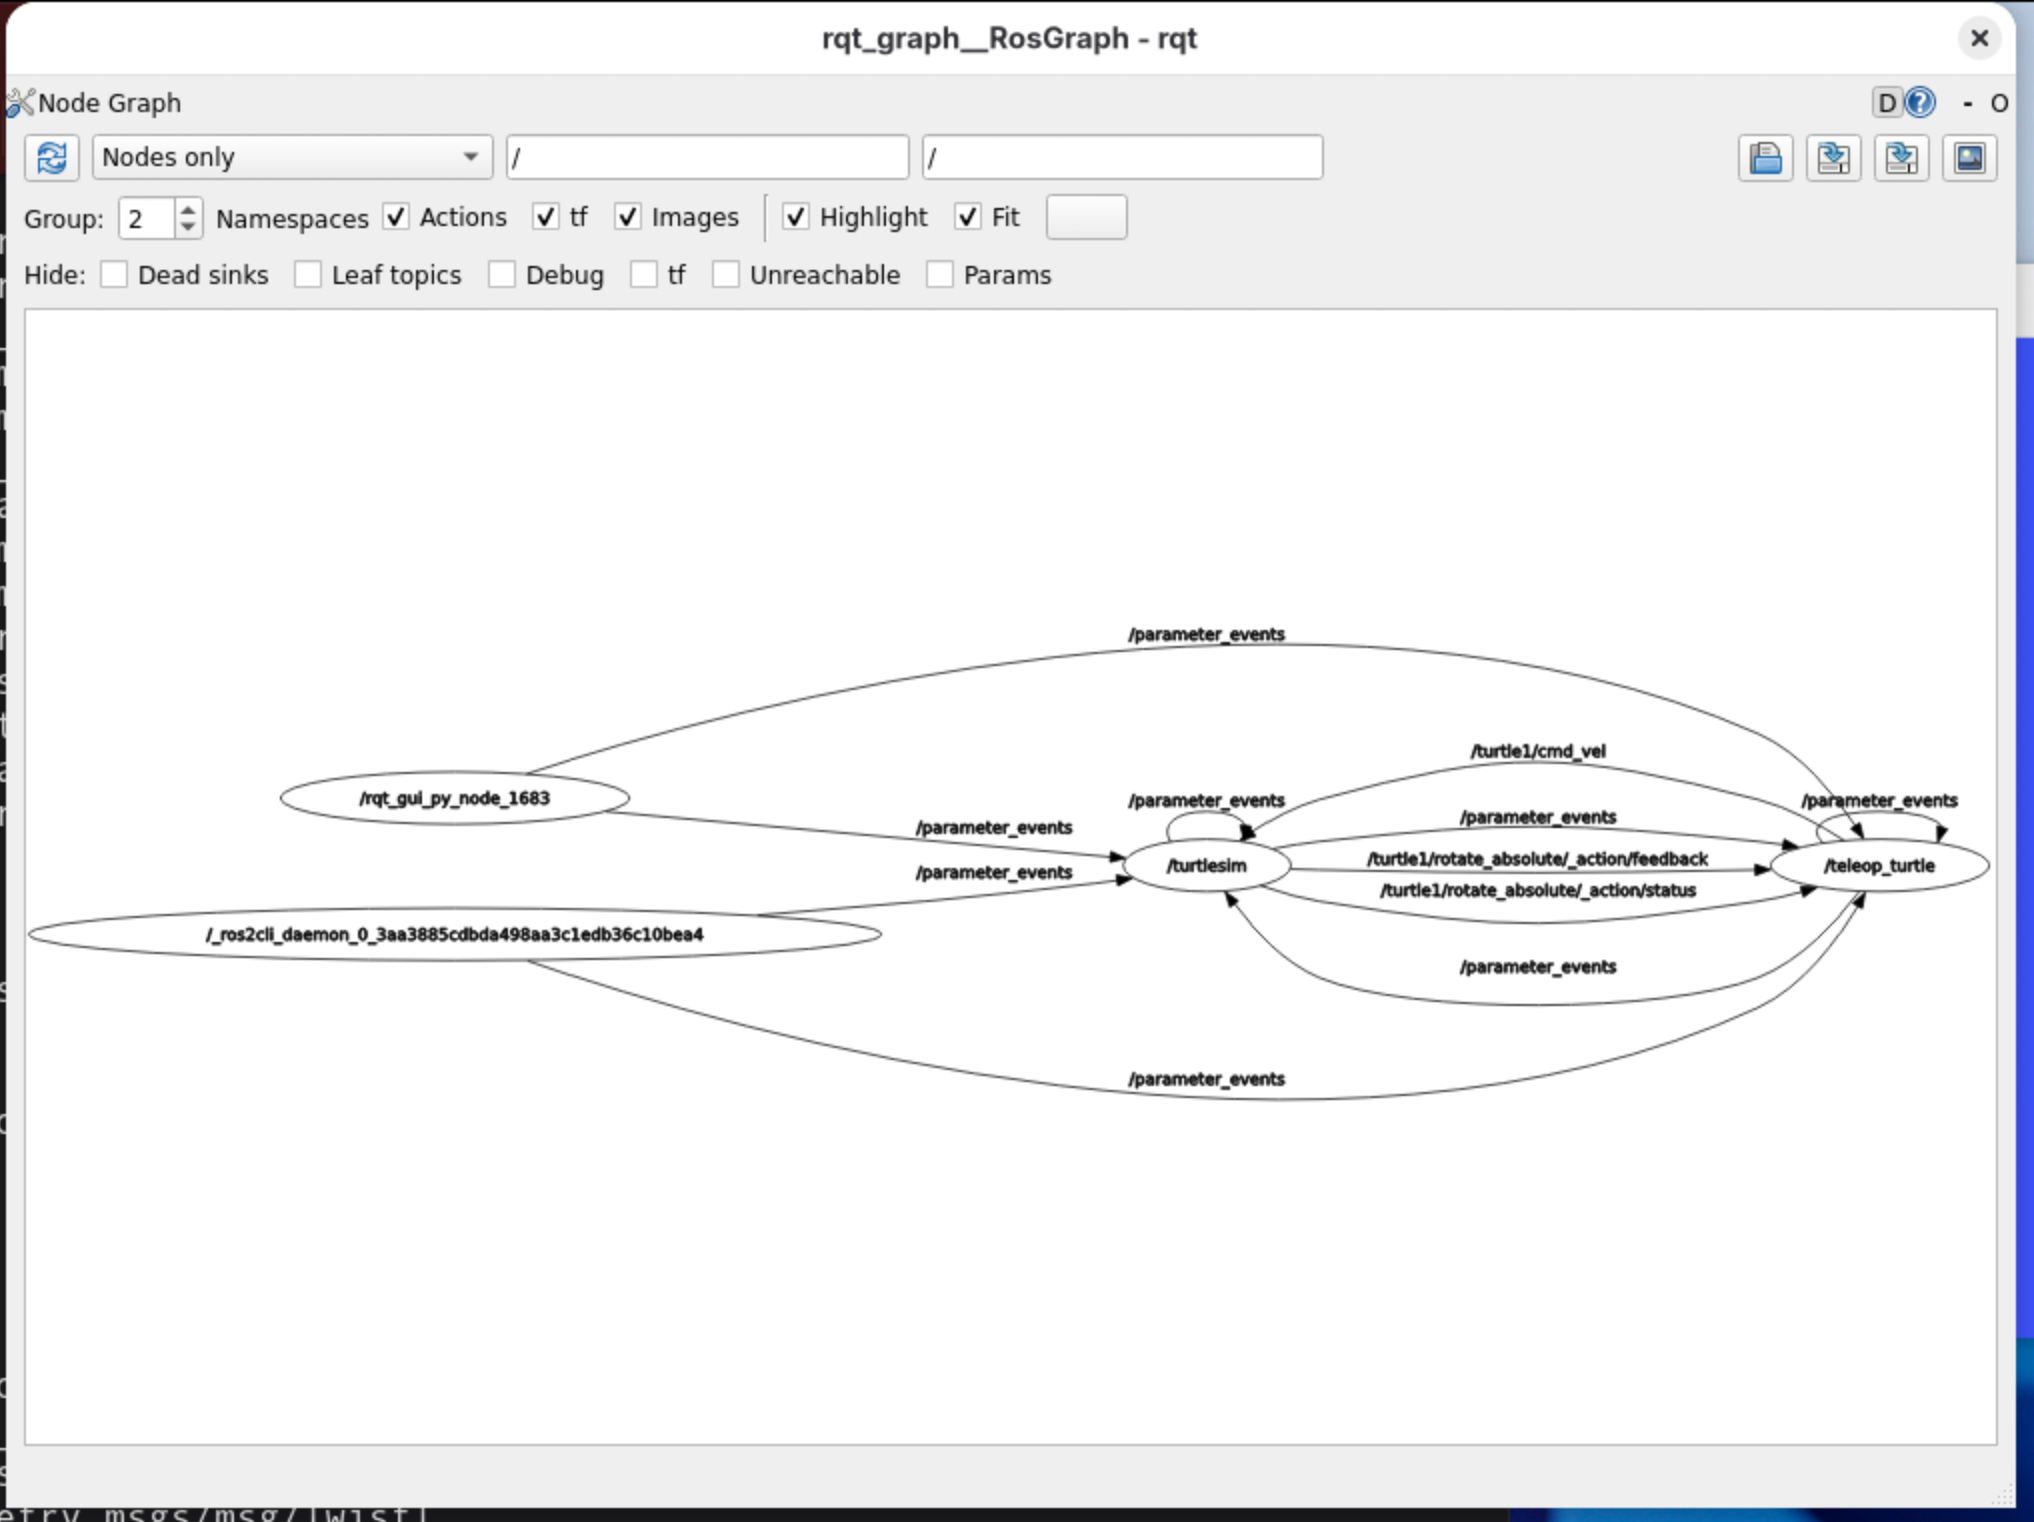
\includegraphics[width=0.75\textwidth]{p1.4-4}
\end{figure}
\item ros2 topic echo
\begin{lstlisting}[language=bash]
ros2 topic echo /turtle1/cmd_vel
\end{lstlisting}
And we can see the data published to the topic \texttt{/turtle1/cmd\_vel}:
\begin{figure}[h]
	\setlength{\leftskip}{2.4em}
	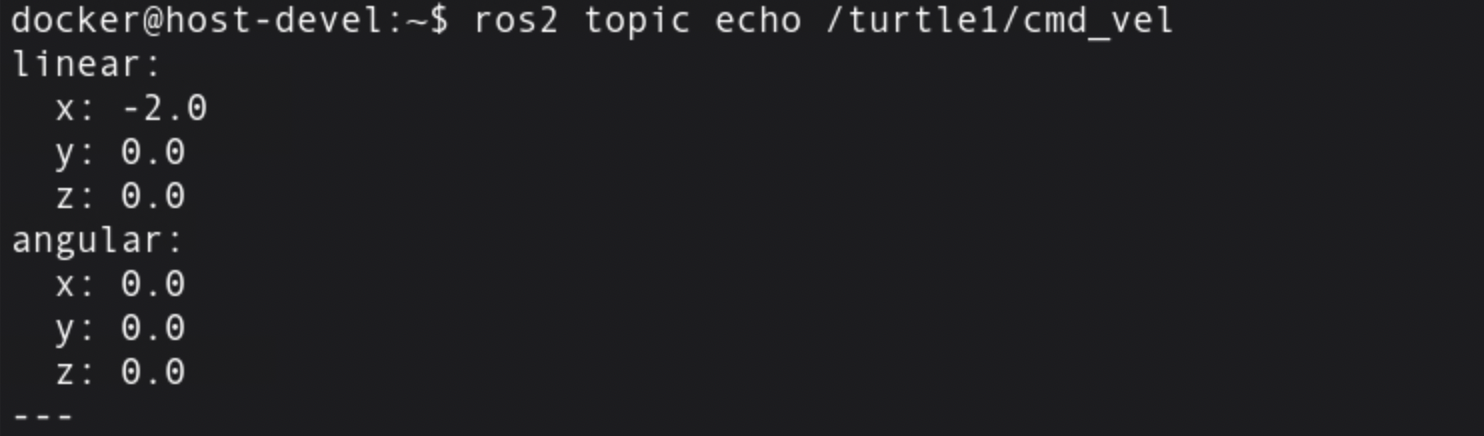
\includegraphics[width=0.94\textwidth]{p1.4-5}
\end{figure}

Uncheck the Debug box on \texttt{rqt\_graph}, we can see that \texttt{/\_ros2cli\_1739} is created by previous command, and there are two nodes subscribed to \texttt{/turtle1/cmd\_vel}:
\begin{figure}[h]
	\setlength{\leftskip}{2.4em}
	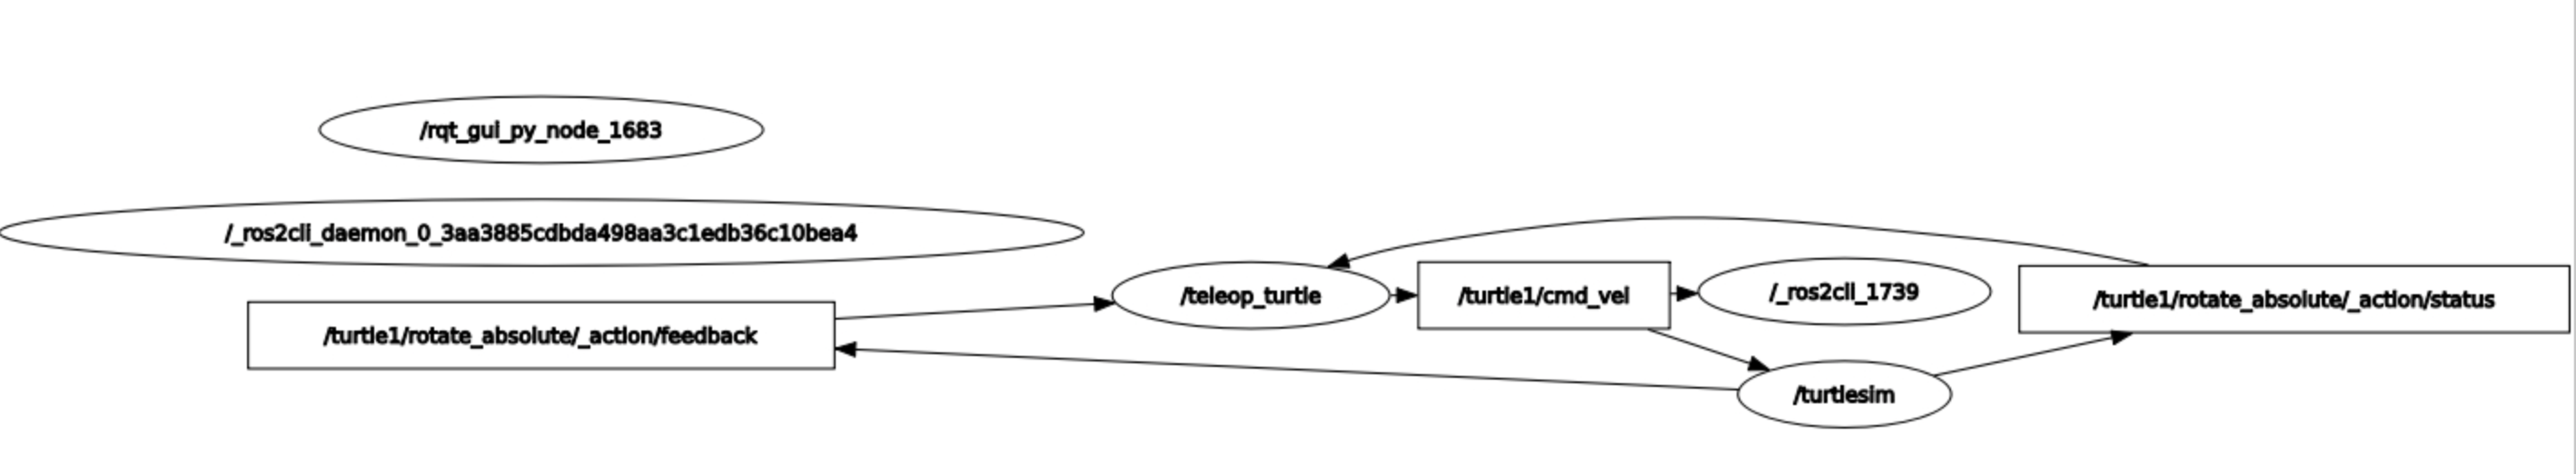
\includegraphics[width=0.94\textwidth]{p1.4-6}
\end{figure}

\newpage
\item ros2 topic info
\begin{lstlisting}[language=bash]
ros2 topic info /turtle1/cmd_vel
\end{lstlisting}
\begin{figure}[h]
	\setlength{\leftskip}{2.4em}
	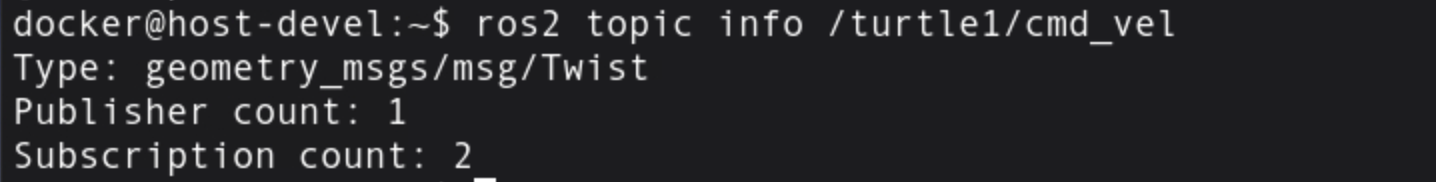
\includegraphics[width=0.94\textwidth]{p1.4-7}
\end{figure}
It returns the information including the amount of publishers and subscriptions of \texttt{/turtle1/cmd\_vel}.
\item ros2 interface show
\begin{lstlisting}[language=bash]
ros2 interface show geometry_msgs/msg/Twist
\end{lstlisting}
It shows the detail of the type "\texttt{geometry\_msgs/msg/Twist".}
\begin{figure}[h]
	\setlength{\leftskip}{2.4em}
	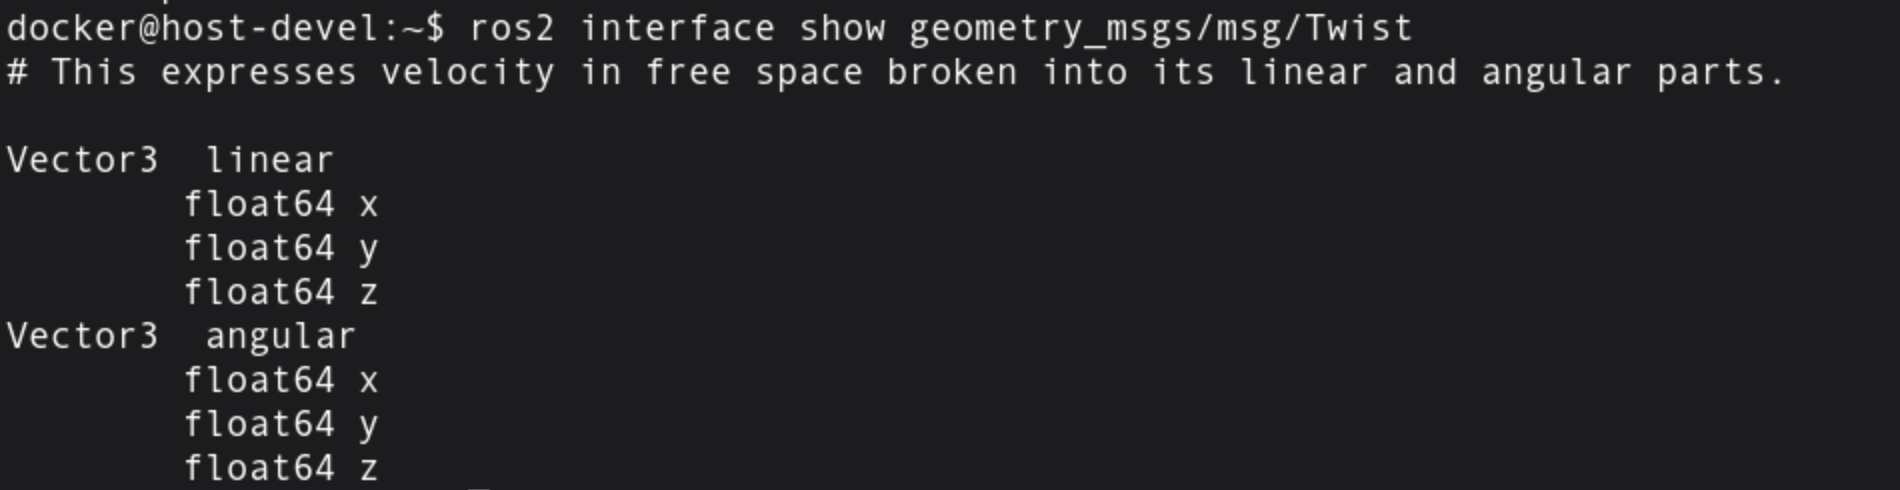
\includegraphics[width=0.94\textwidth]{p1.4-8}
\end{figure}
\item ros2 topic pub\\
I can directly publish a data to a topic by command:
\begin{lstlisting}[language=bash]
ros2 topic pub /turtle1/cmd_vel geometry_msgs/msg/Twist "{linear: {x: 2.0, y: 0.0, z: 0.0}, angular: {x: 0.0, y: 0.0, z: 1.8}}"
\end{lstlisting}
With no other options, it will publish in a steady stream 1Hz.
\begin{figure}[h]
	\setlength{\leftskip}{2.4em}
	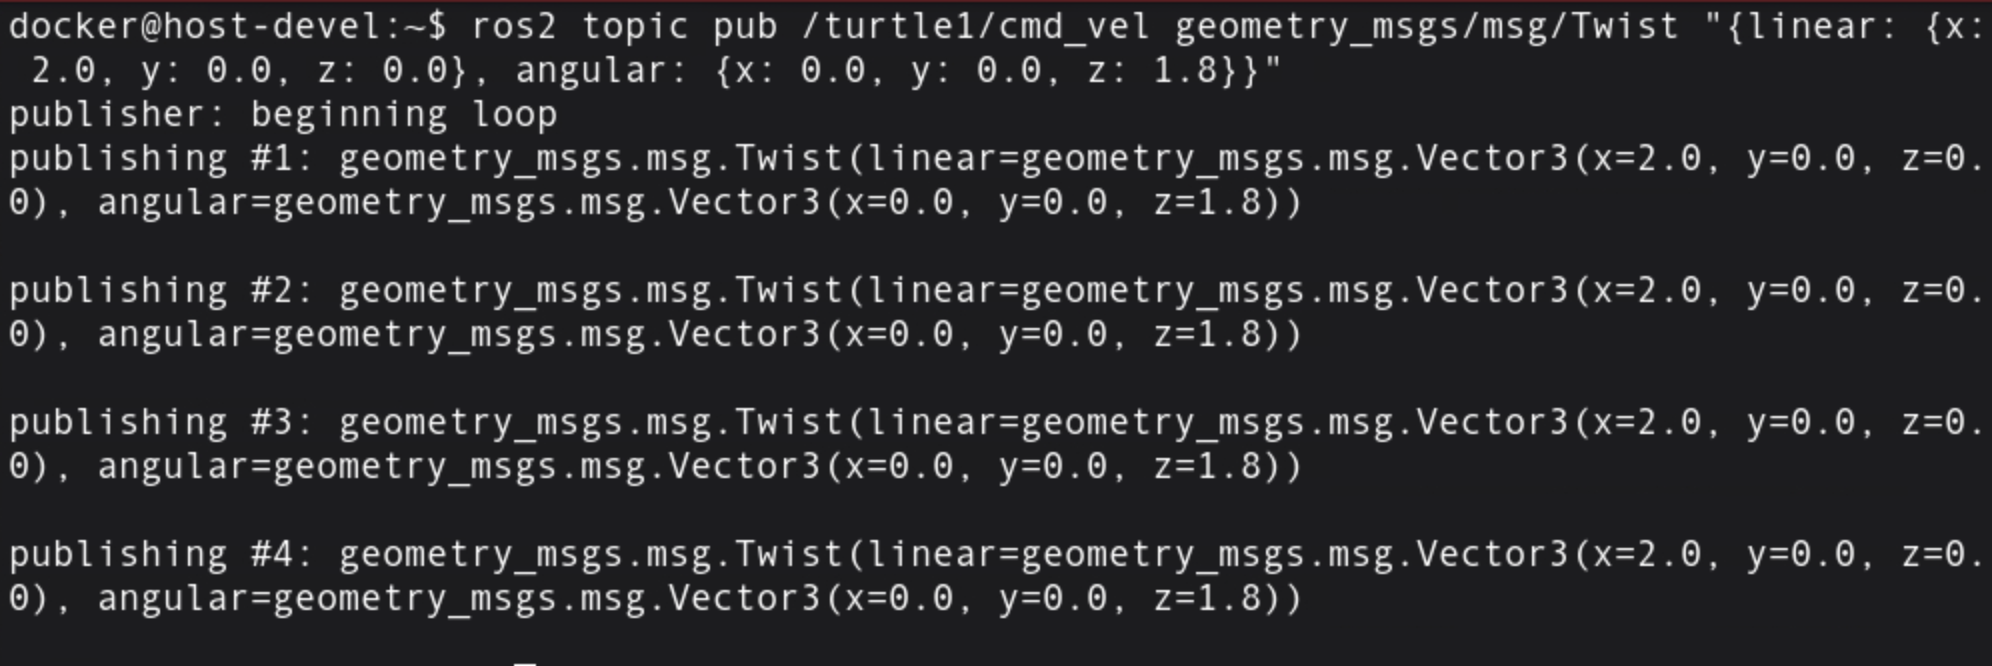
\includegraphics[width=0.94\textwidth]{p1.4-9}
\end{figure}
\begin{figure}[h]
	\centering
	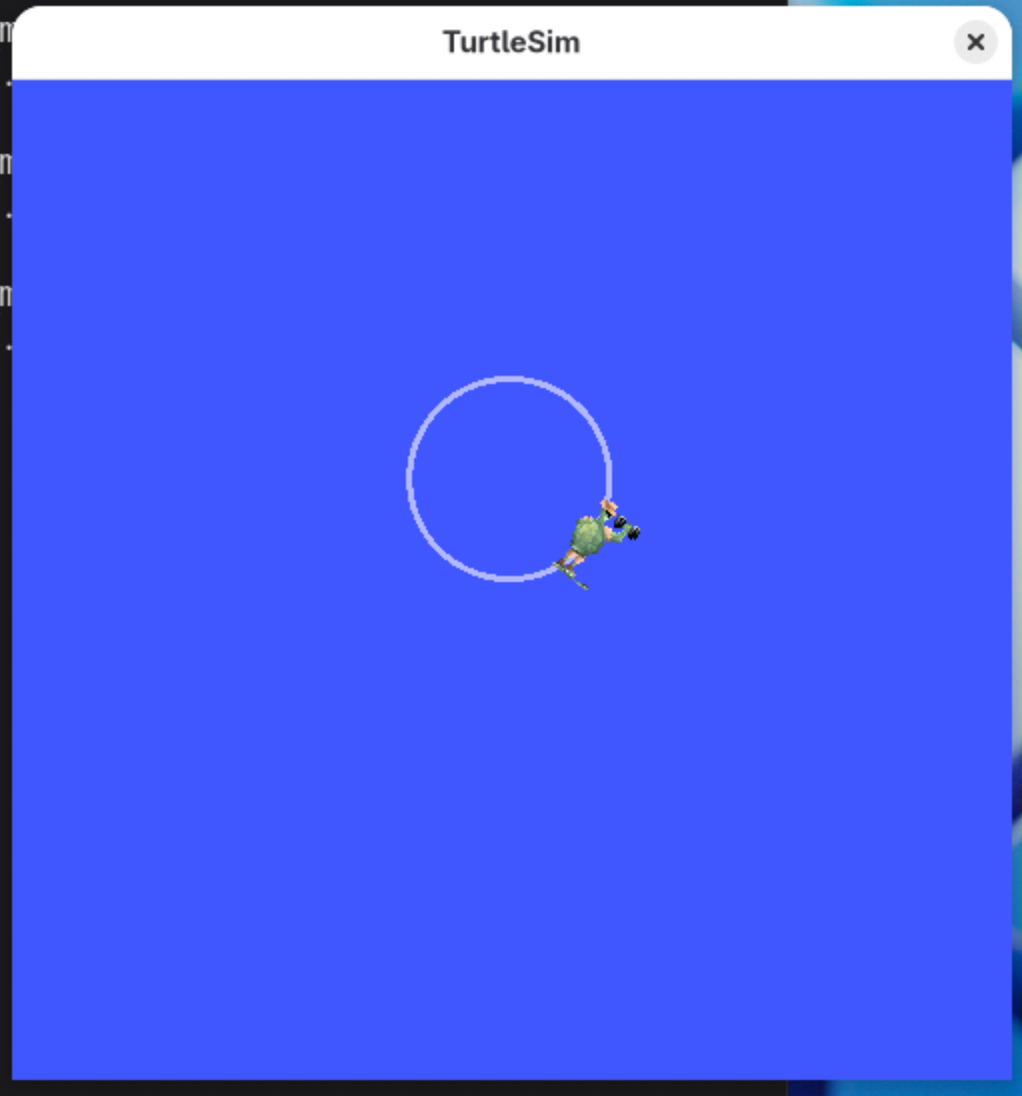
\includegraphics[width=0.4\textwidth]{p1.4-10}
\end{figure}
\newpage
By using \texttt{--once}(publish one message then exit) and  \texttt{-w 2}(wait for 2 matching subscriptions):
\begin{lstlisting}[language=bash]
ros2 topic pub /turtle1/cmd_vel geometry_msgs/msg/Twist "{linear: {x: 2.0, y: 0.0, z: 0.0}, angular: {x: 0.0, y: 0.0, z: 1.8}}" --once -w 2
\end{lstlisting}
\begin{figure}[h]
	\setlength{\leftskip}{2.4em}
	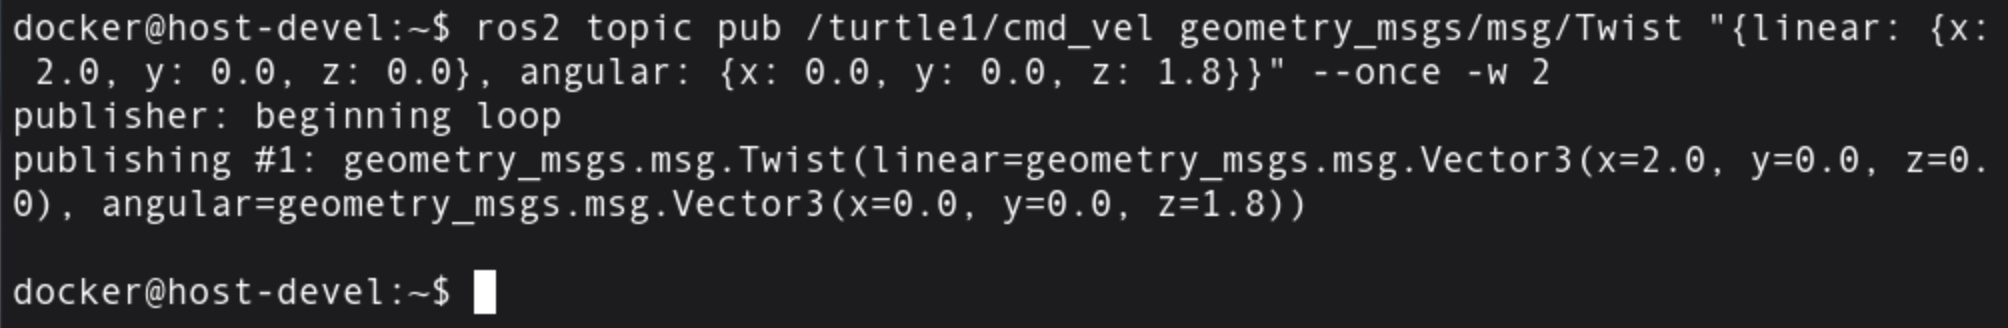
\includegraphics[width=0.94\textwidth]{p1.4-11}
\end{figure}
\begin{figure}[h]
	\centering
	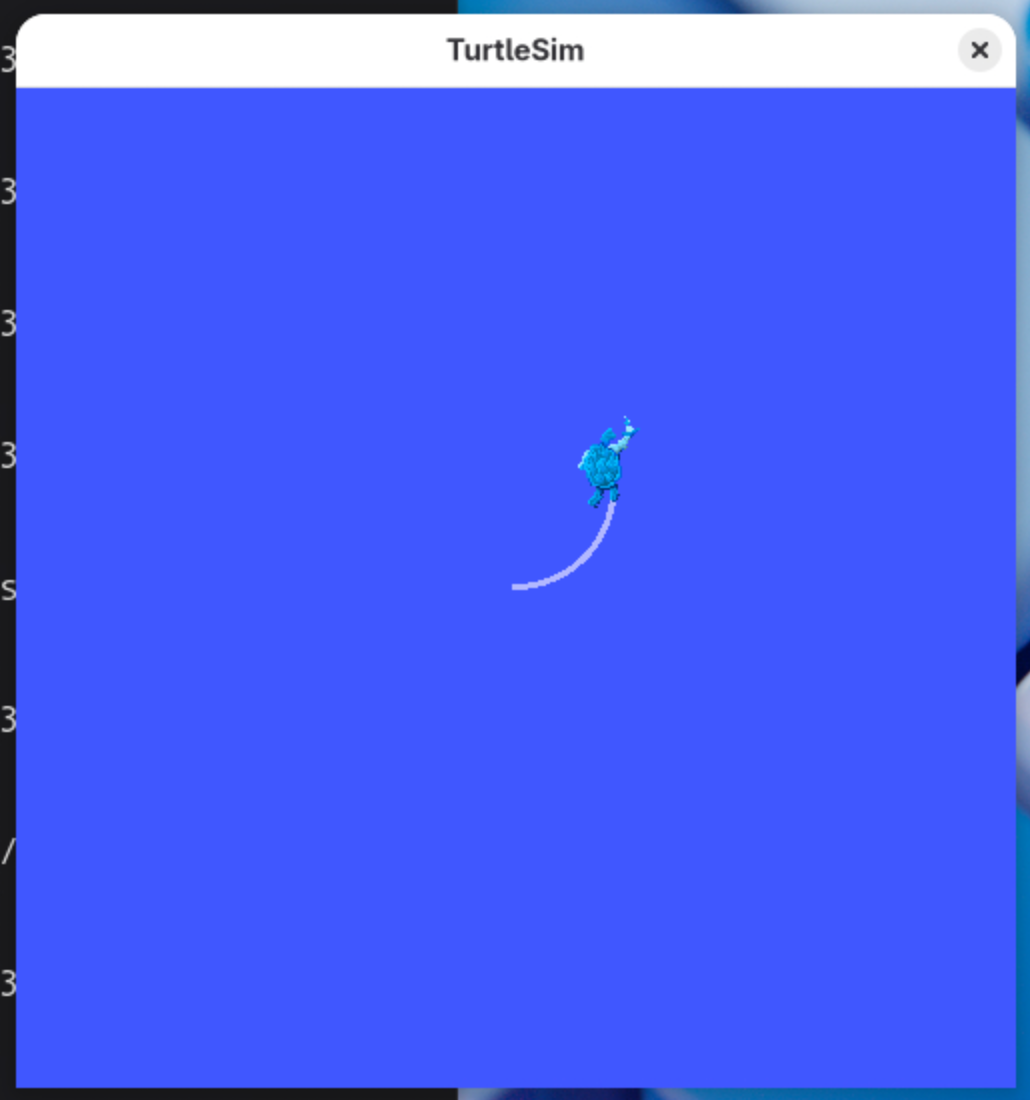
\includegraphics[width=0.4\textwidth]{p1.4-12}
\end{figure}


\newpage
Refresh the \texttt{rqt\_graph}, and we can see that the node \texttt{/\_ros2cli\_2147}(\texttt{ros2 topic pub...}) also published data to the topic \texttt{/turtle1/cmd\_vel}:
\begin{figure}[h]
	\setlength{\leftskip}{2.4em}
	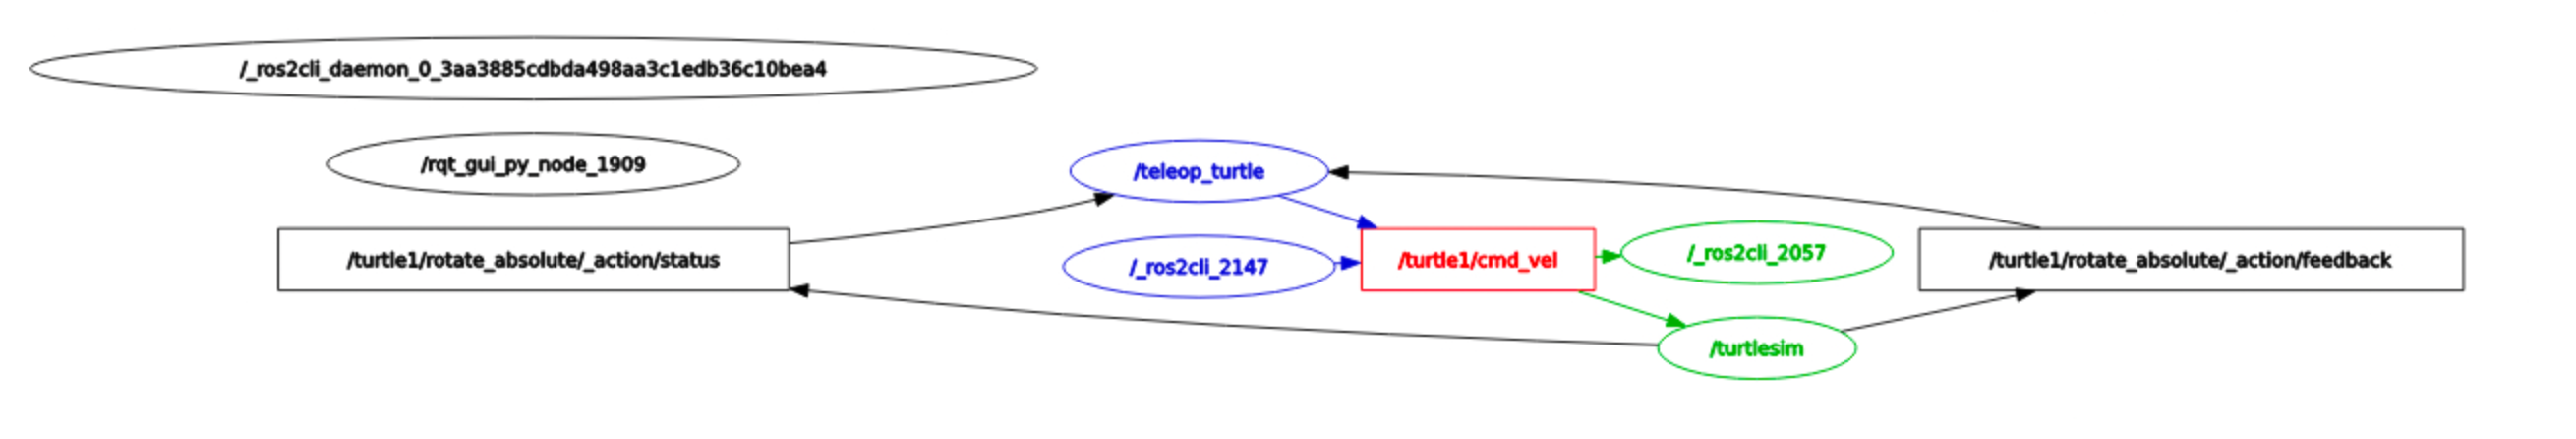
\includegraphics[width=0.94\textwidth]{p1.4-13}
\end{figure}


Run \texttt{echo} on the \texttt{pose} topic and recheck \texttt{rqt\_graph}:
\begin{figure}[h]
	\setlength{\leftskip}{2.4em}
	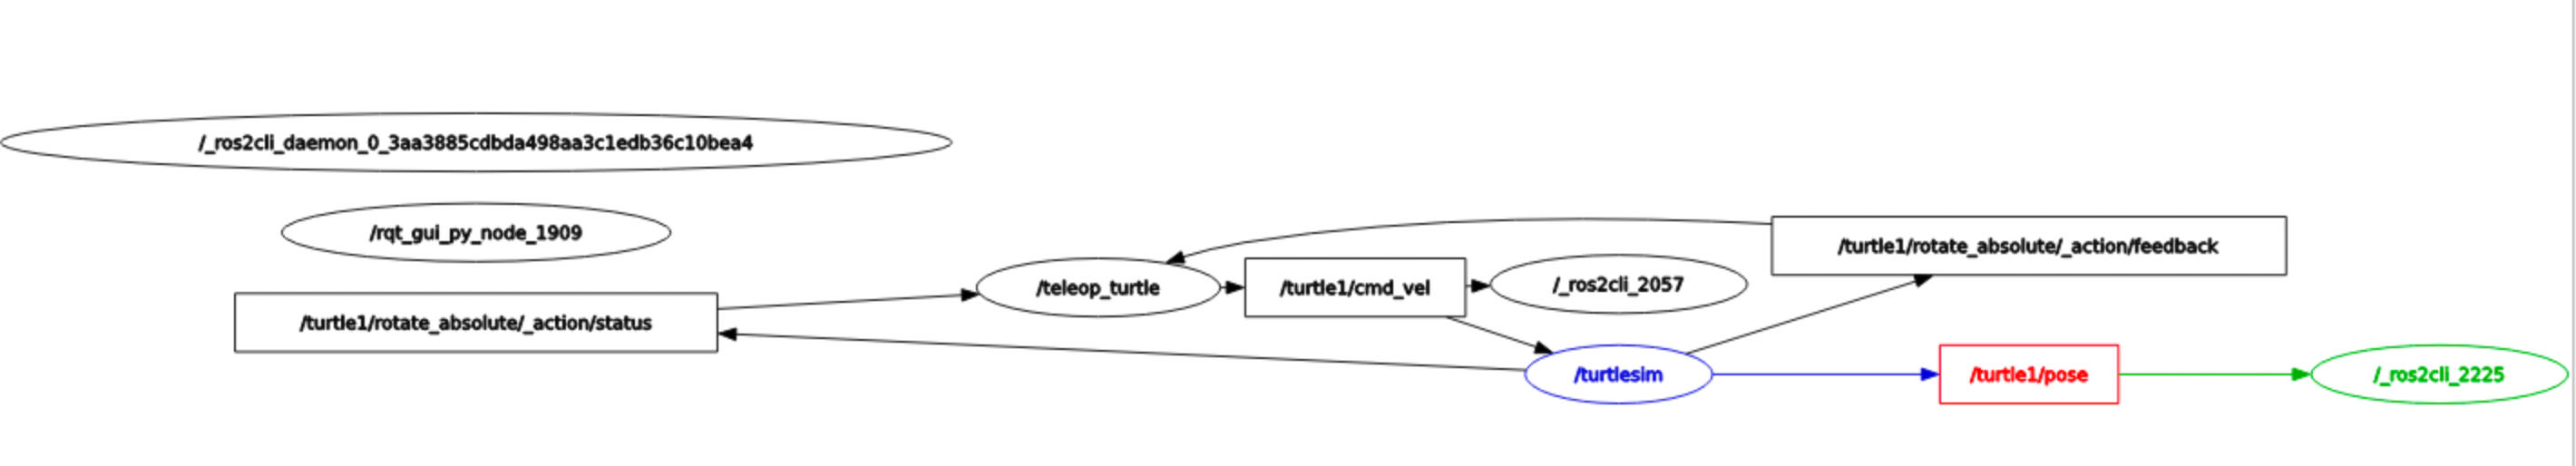
\includegraphics[width=0.94\textwidth]{p1.4-14}
\end{figure}
We can see that \texttt{/turtlesim} also publishing to the topic \texttt{/turtle1/pose}, which the new \texttt{echo} node\\(\texttt{/\_ros2cli\_2225}) subscribed to.

\item ros2 topic hz\\
	We can see the rate at which data is published:
\begin{lstlisting}[language=bash]
ros2 topic hz /turtle1/pose
\end{lstlisting}
\begin{figure}[h]
	\setlength{\leftskip}{2.4em}
	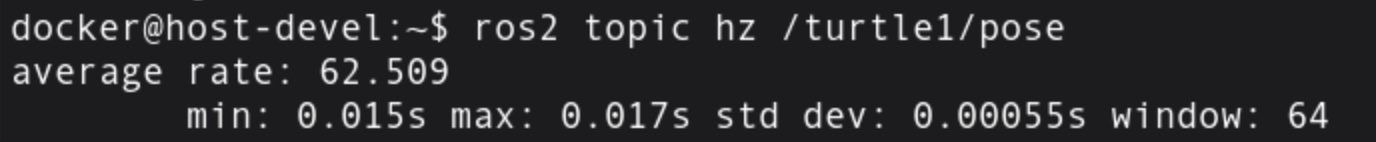
\includegraphics[width=0.94\textwidth]{p1.4-15}
\end{figure}

\newpage
\item ros2 topic bw\\
To view the bandwith of a topic:
\begin{lstlisting}[language=bash]
ros2 topic bw /turtle1/pose
\end{lstlisting}
\begin{figure}[h]
	\setlength{\leftskip}{2.4em}
	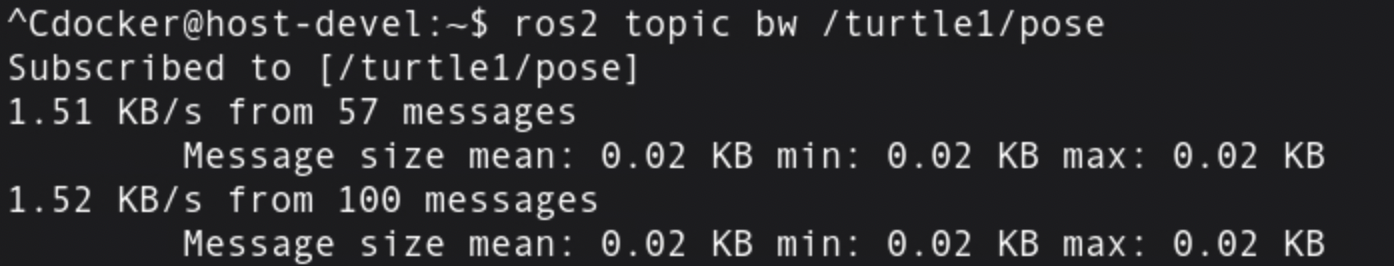
\includegraphics[width=0.94\textwidth]{p1.4-16}
\end{figure}

\item ros2 topic find
Give the topics available for specific type of messages:
\begin{lstlisting}[language=bash]
ros2 topic find geometry_msgs/msg/Twist
\end{lstlisting}
\begin{figure}[h]
	\setlength{\leftskip}{2.4em}
	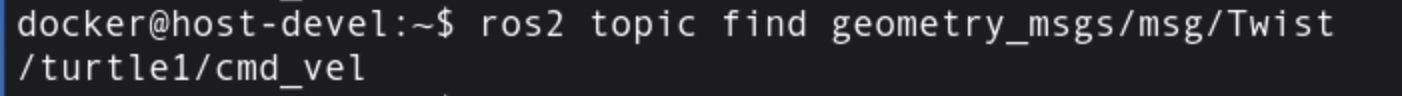
\includegraphics[width=0.94\textwidth]{p1.4-17}
\end{figure}
\item Clean up\\
Use \texttt{Ctrl+C} to clean up all terminals.

\end{enumerate}

\newpage
\subsection{Understanding services}
\begin{enumerate}
	\item Setup
\begin{lstlisting}[language=bash]
ros2 run turtlesim turtlesim_node
ros2 run turtlesim turtle_teleop_key
\end{lstlisting}
\item ros2 service list\\
To see current active services:
\begin{lstlisting}[language=bash]
ros2 service list
\end{lstlisting}
\begin{figure}[h]
	\centering
	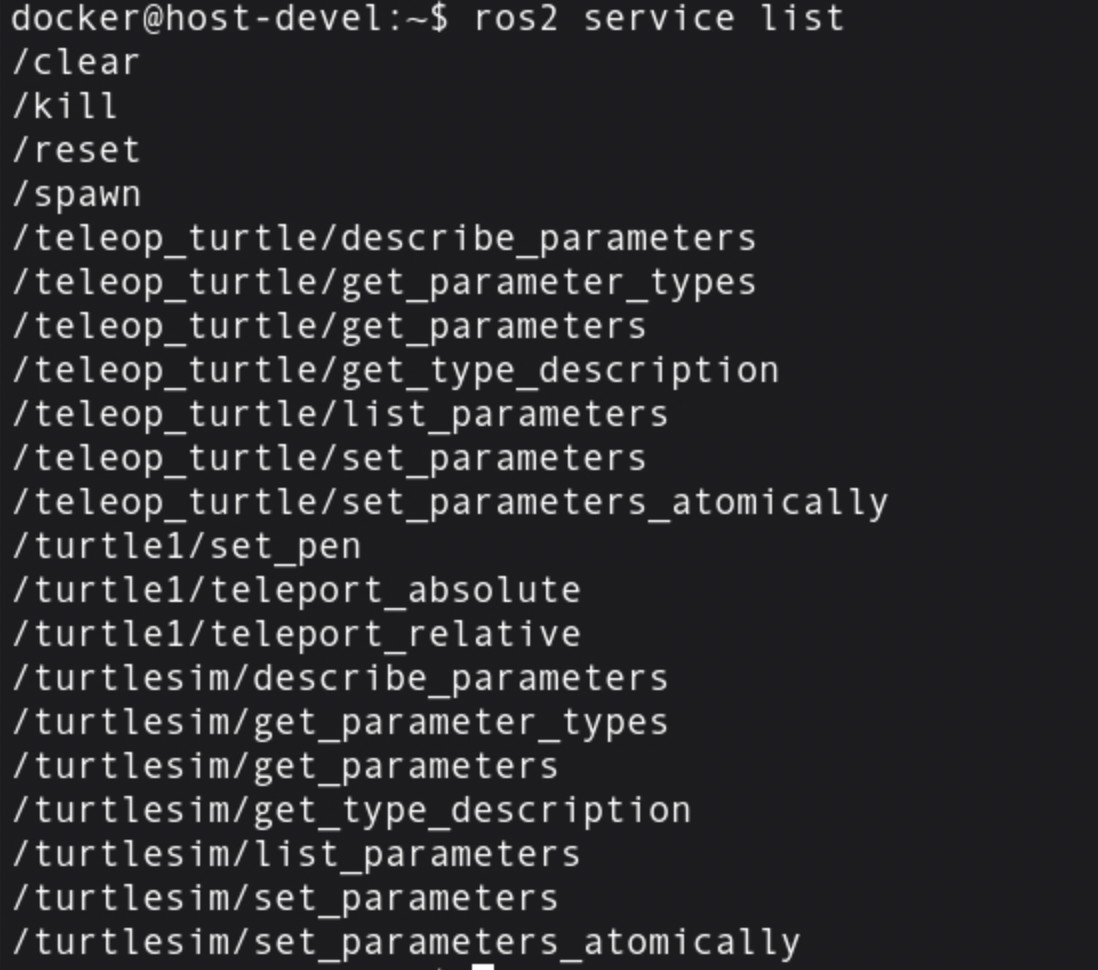
\includegraphics[width=0.75\textwidth]{p1.5-1}
\end{figure}
To see the type of a service:
\begin{lstlisting}[language=bash]
ros2 service type <service>
\end{lstlisting}
e.g. the type of \texttt{/kill}:
\begin{figure}[h]
	\setlength{\leftskip}{2.4em}
	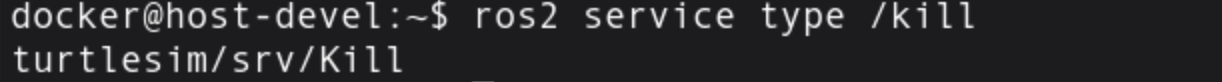
\includegraphics[width=0.94\textwidth]{p1.5-2}
\end{figure}

\newpage
\begin{itemize}
	\item ros2 service list -t\\
Similar to \texttt{topic}, we can add the option \texttt{-t}, to see the types of all services.
\begin{lstlisting}[language=bash]
ros2 service list -t
\end{lstlisting}
\begin{figure}[h]
	\centering
	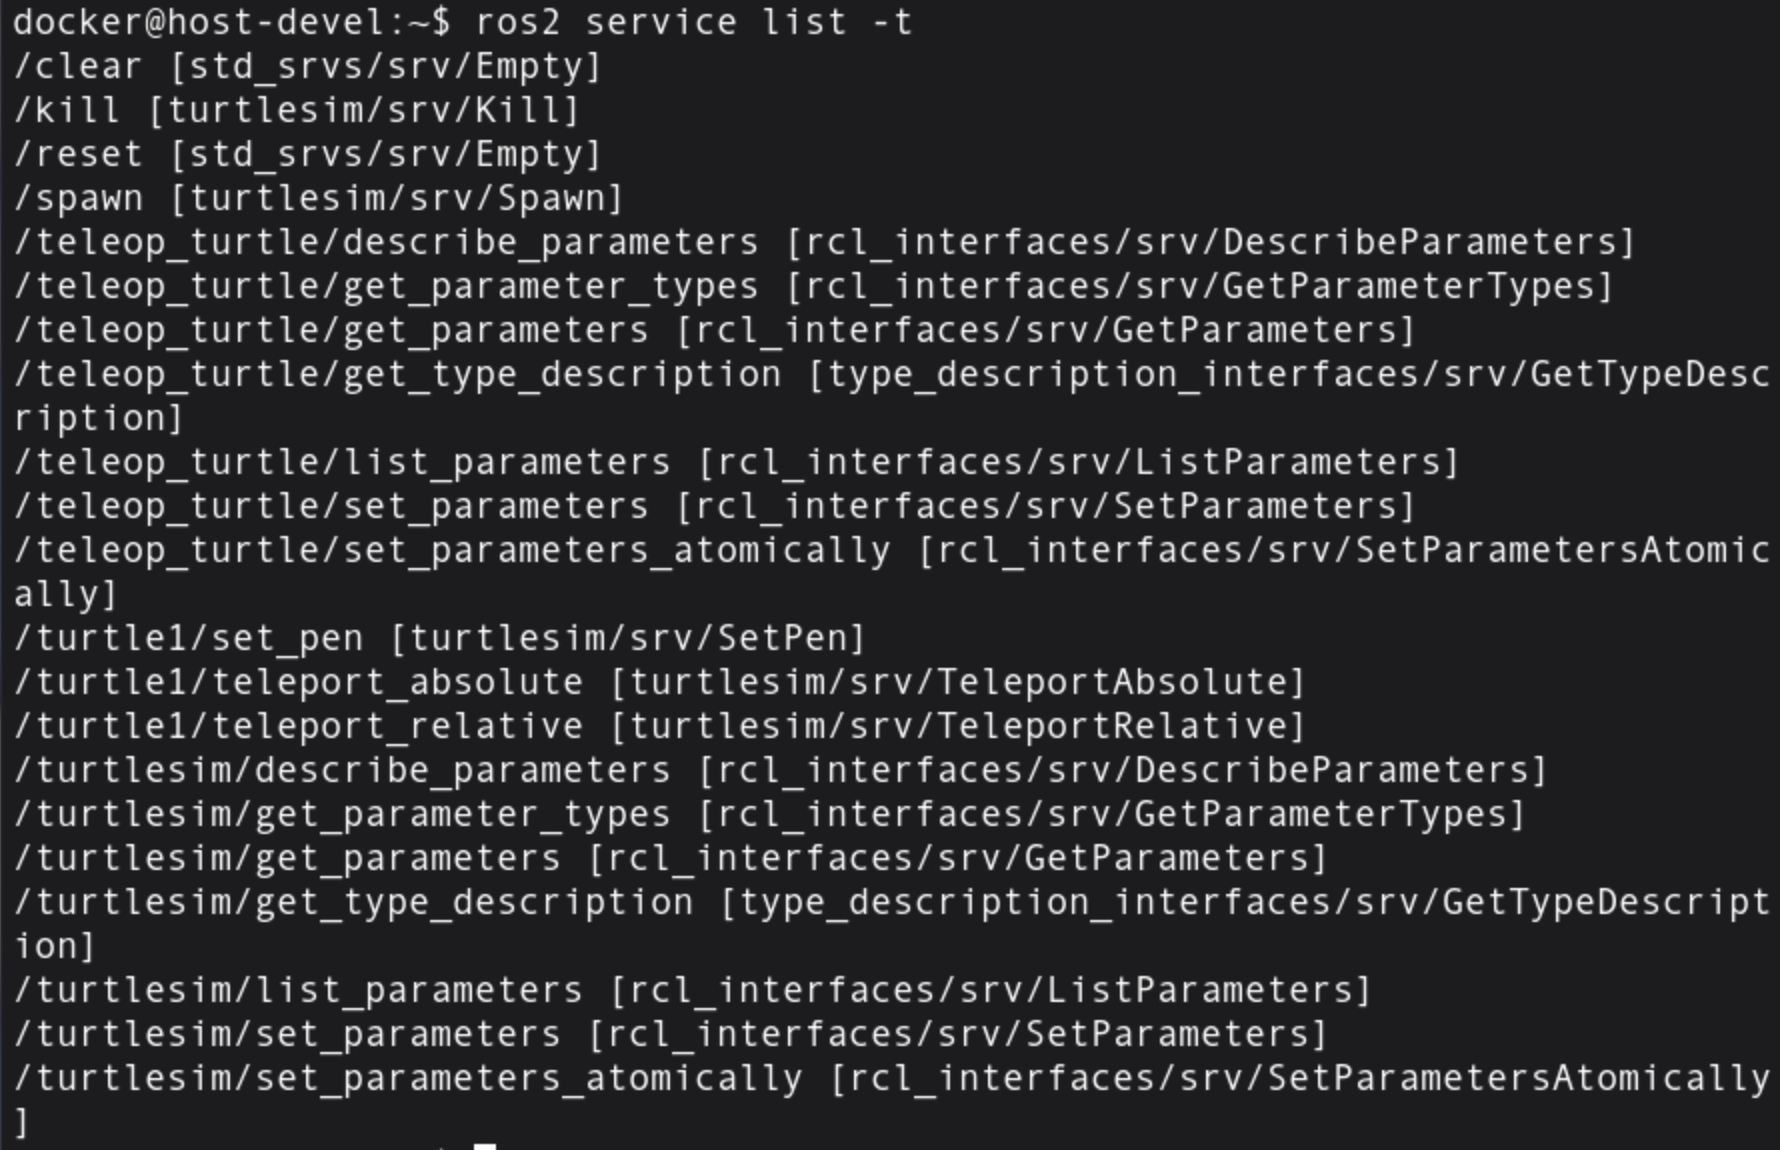
\includegraphics[width=0.75\textwidth]{p1.5-3}
\end{figure}
\end{itemize}

\item ros2 service find\\
Find all services of a specific type:
\begin{lstlisting}[language=bash]
ros2 service find std_srvs/srv/Empty
\end{lstlisting}
\begin{figure}[h]
	\setlength{\leftskip}{2.4em}
	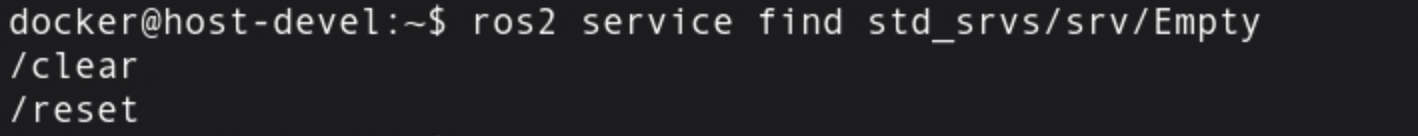
\includegraphics[width=0.94\textwidth]{p1.5-4}
\end{figure}

\item ros2 interface show\\
Se the detail of a type:
\begin{lstlisting}[language=bash]
ros2 interface show turtlesim/srv/Spawn
\end{lstlisting}
\begin{figure}[h]
	\setlength{\leftskip}{2.4em}
	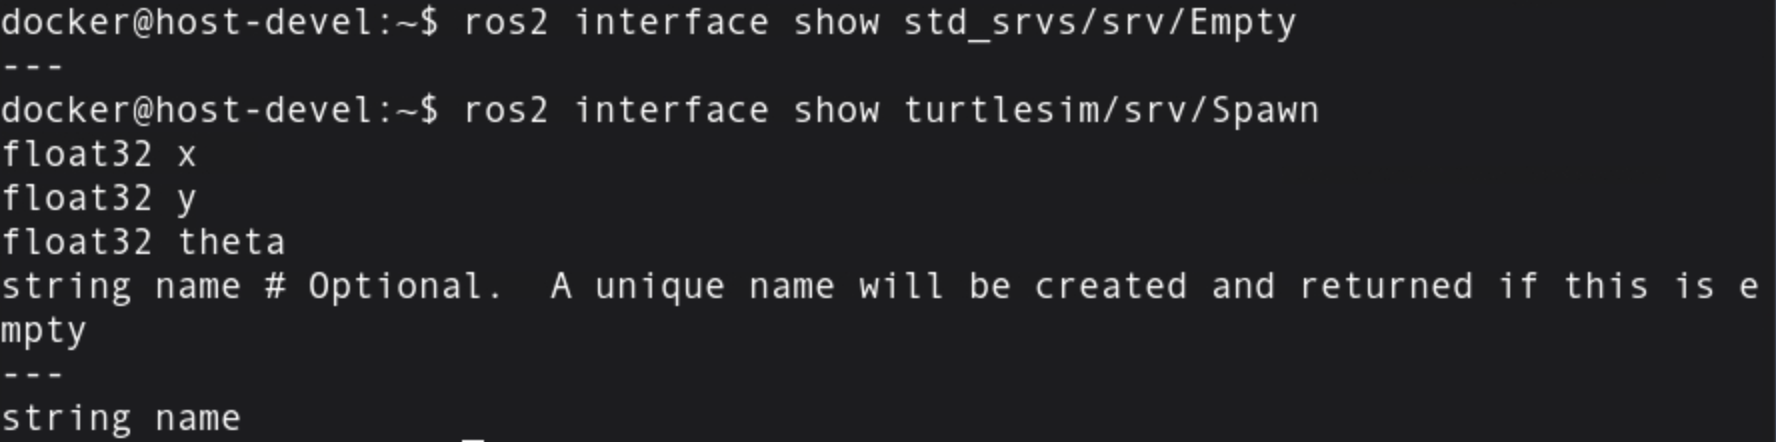
\includegraphics[width=0.94\textwidth]{p1.5-5}
\end{figure}

\newpage
\item ros2 service call\\
Call a service:
\begin{lstlisting}[language=bash]
ros2 service call /clear std_srvs/srv/Empty
\end{lstlisting}
\begin{figure}[h]
	\centering
	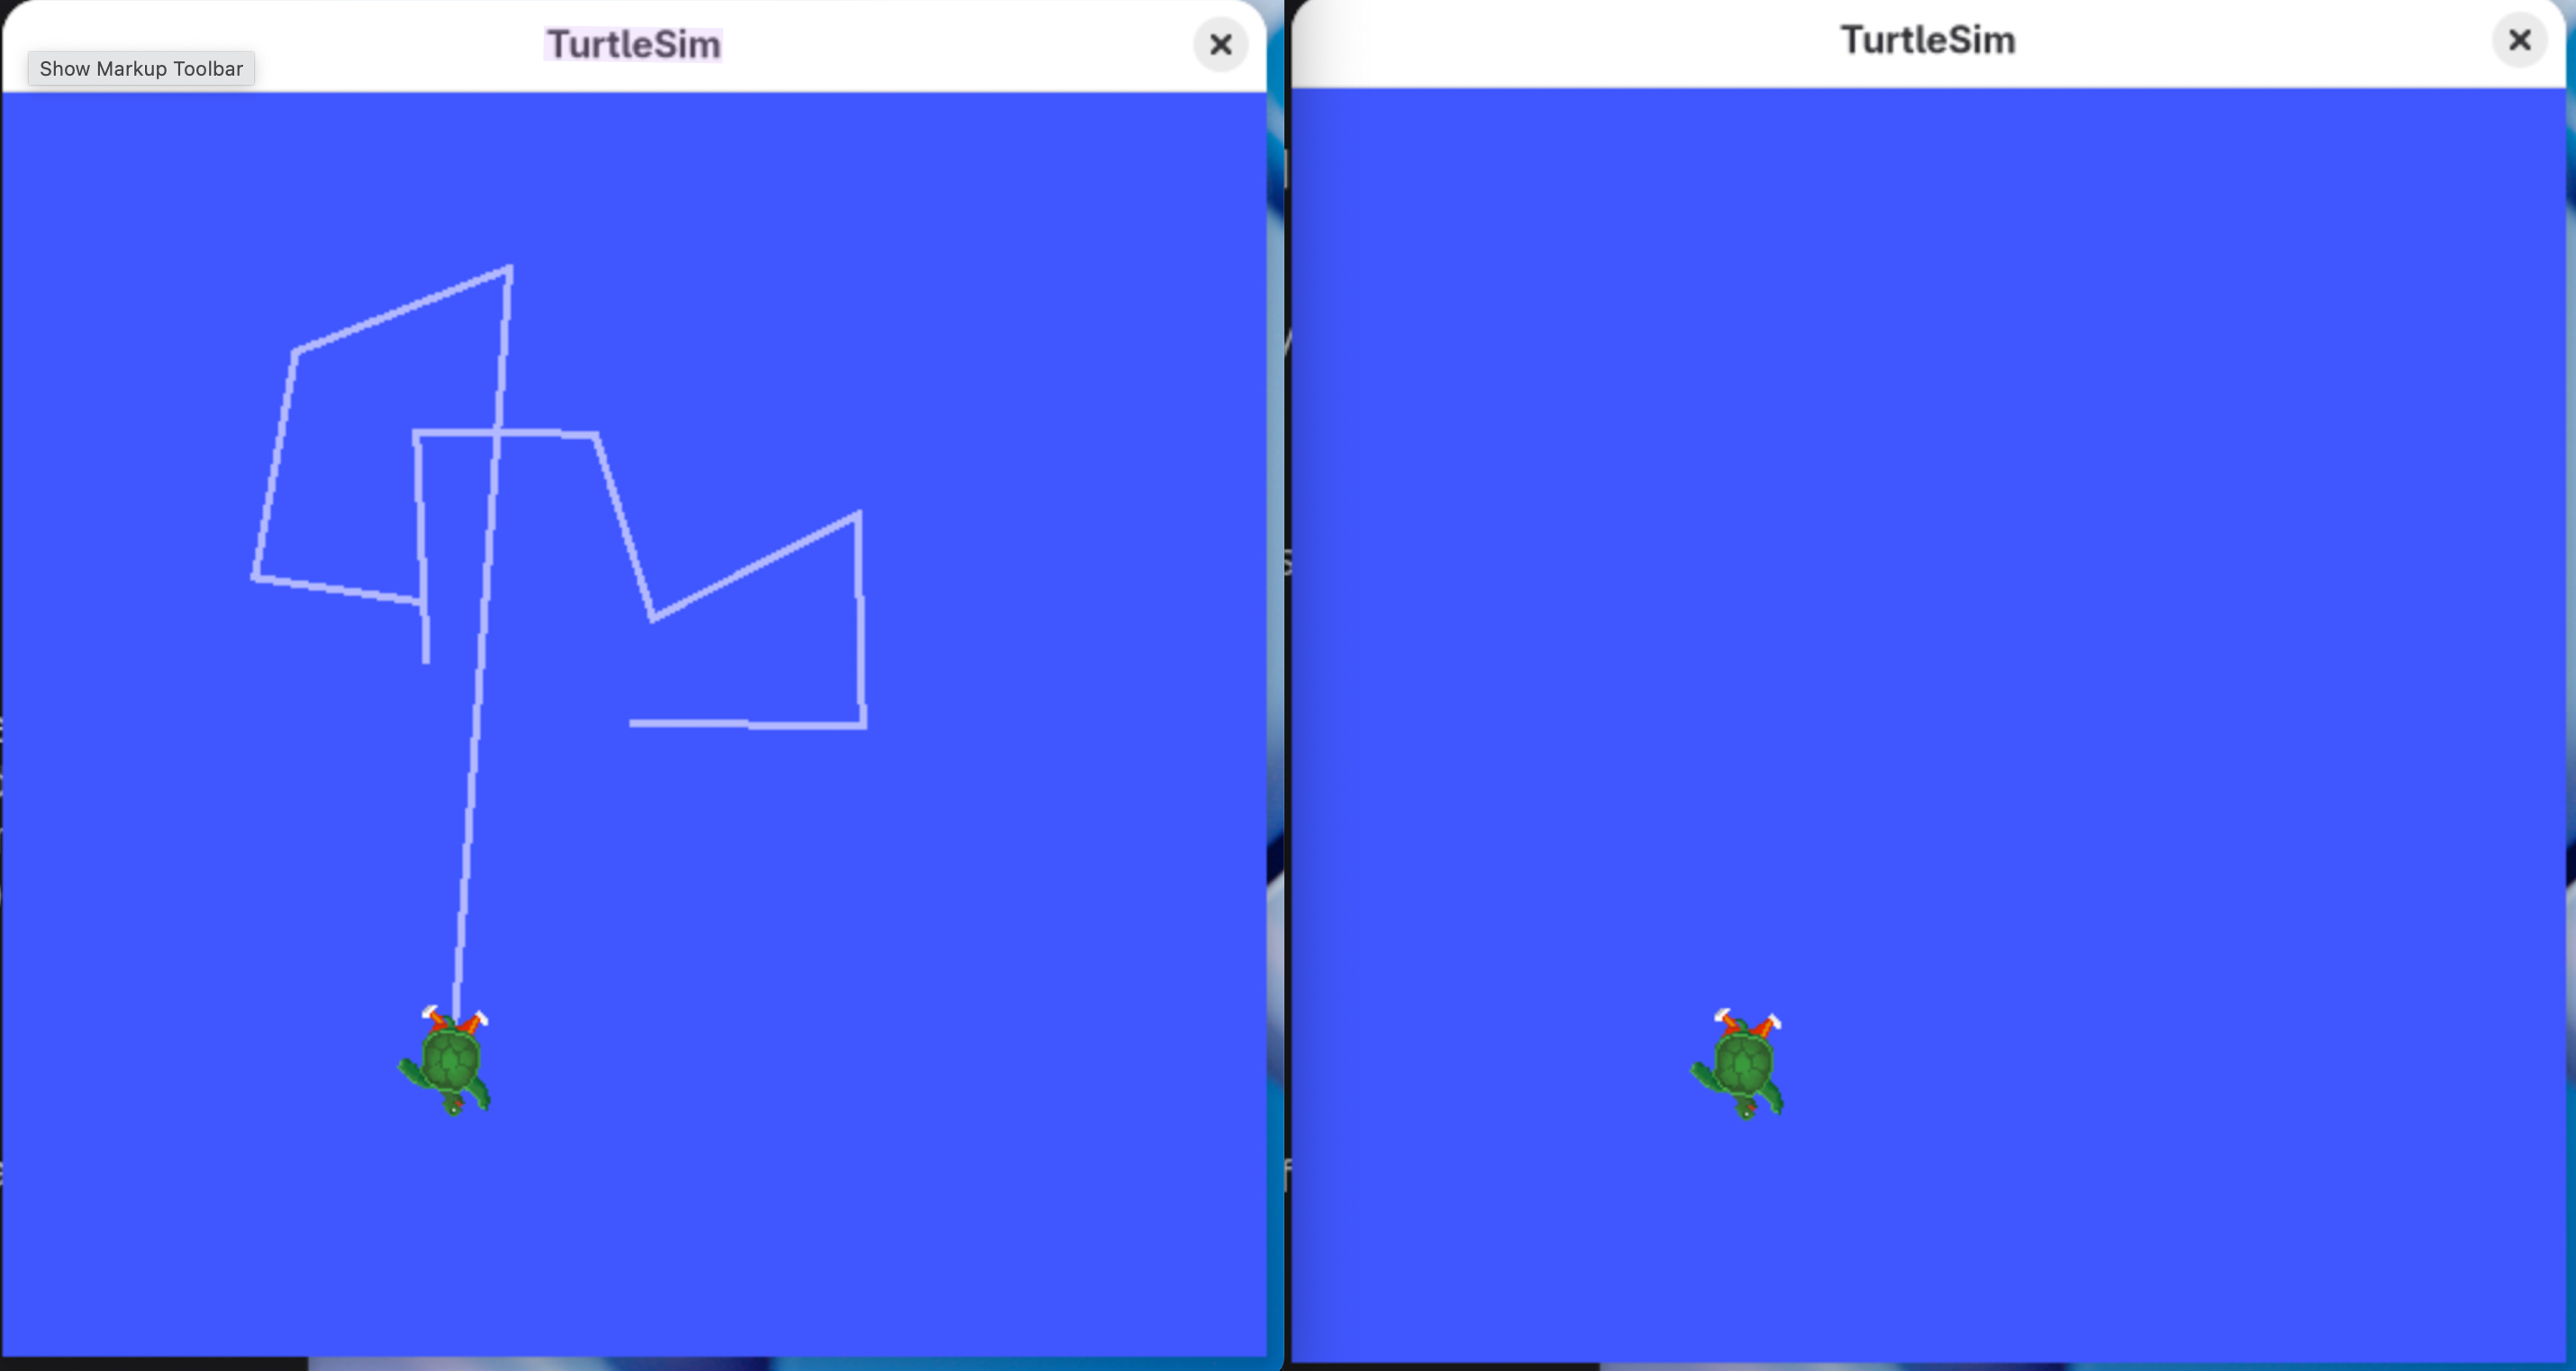
\includegraphics[width=0.75\textwidth]{p1.5-6}
\end{figure}

\begin{lstlisting}[language=bash]
ros2 service call /spawn turtlesim/srv/Spawn "{x: 3, y: 4, theta: 0.5, name: 'hehe'}"
\end{lstlisting}
\begin{figure}[h]
	\setlength{\leftskip}{2.4em}
	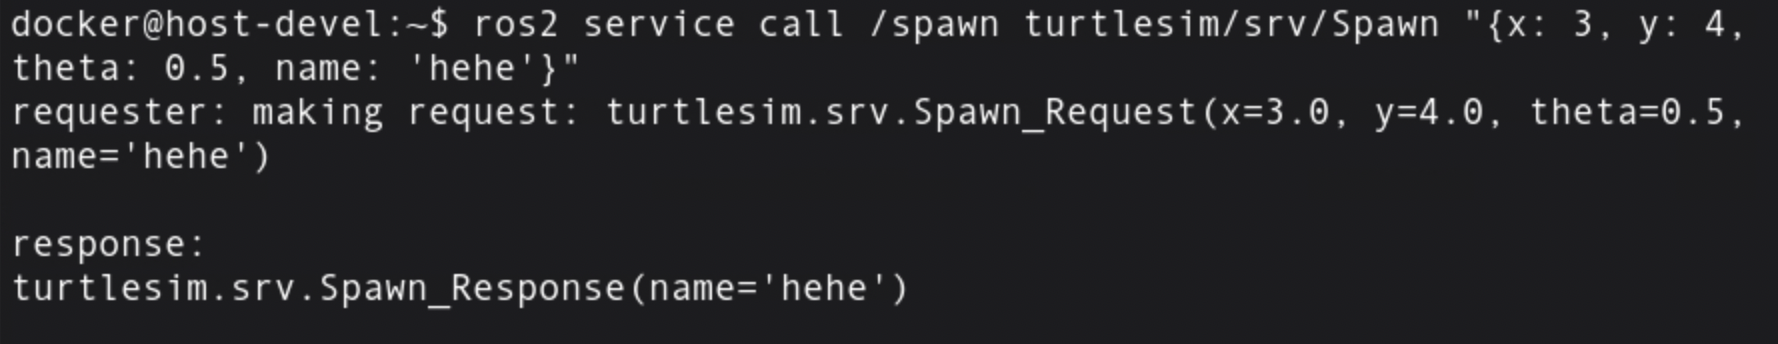
\includegraphics[width=0.94\textwidth]{p1.5-7}
\end{figure}
\begin{figure}[h]
	\centering
	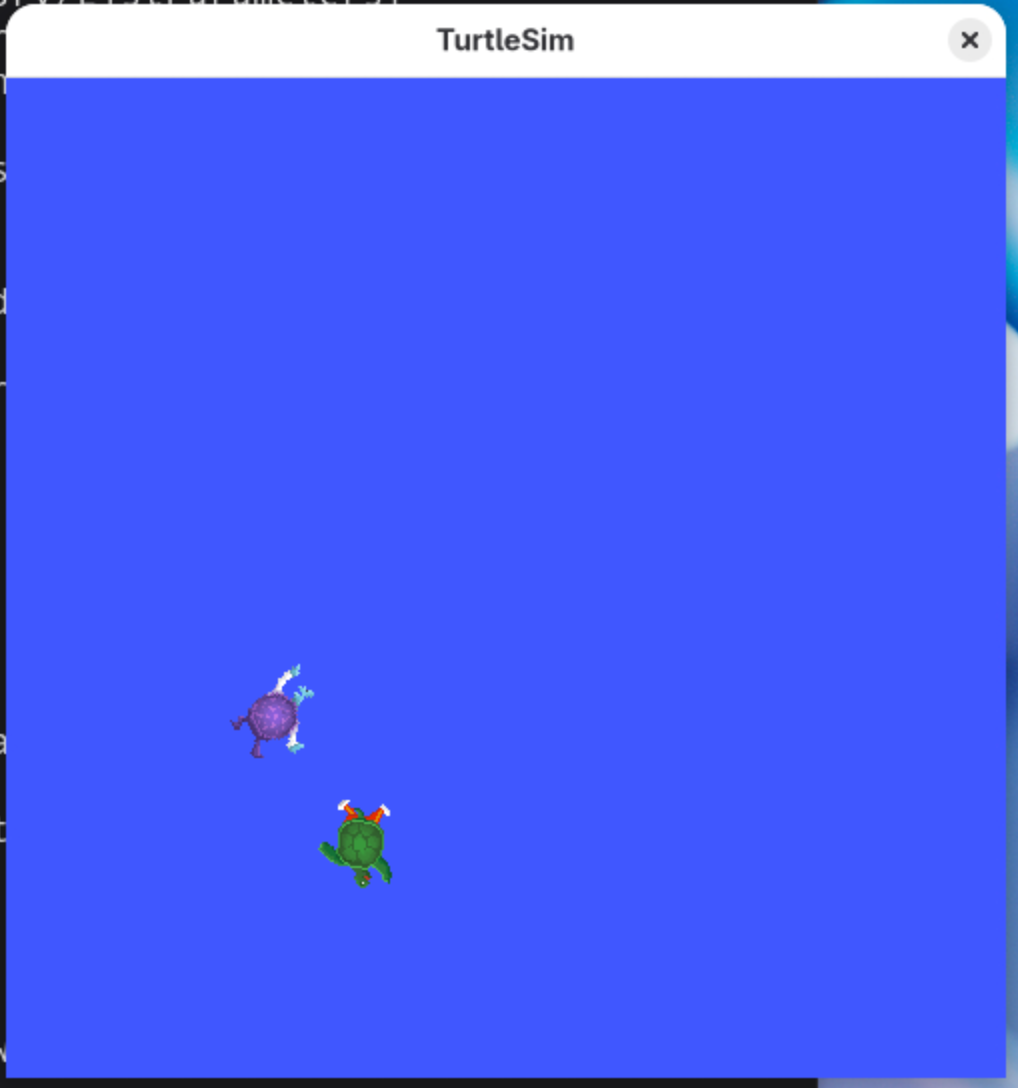
\includegraphics[width=0.4\textwidth]{p1.5-8}
\end{figure}
\end{enumerate}

\newpage
\subsection{Understanding parameters}
\begin{enumerate}
	\item Setup
\begin{lstlisting}[language=bash]
ros2 run turtlesim turtlesim_node
ros2 run turtlesim turtle_teleop_key
\end{lstlisting}
\item ros2 param list\\
To see each node's parameters:
\begin{lstlisting}[language=bash]
ros2 param list
\end{lstlisting}
\begin{figure}[h]
	\centering
	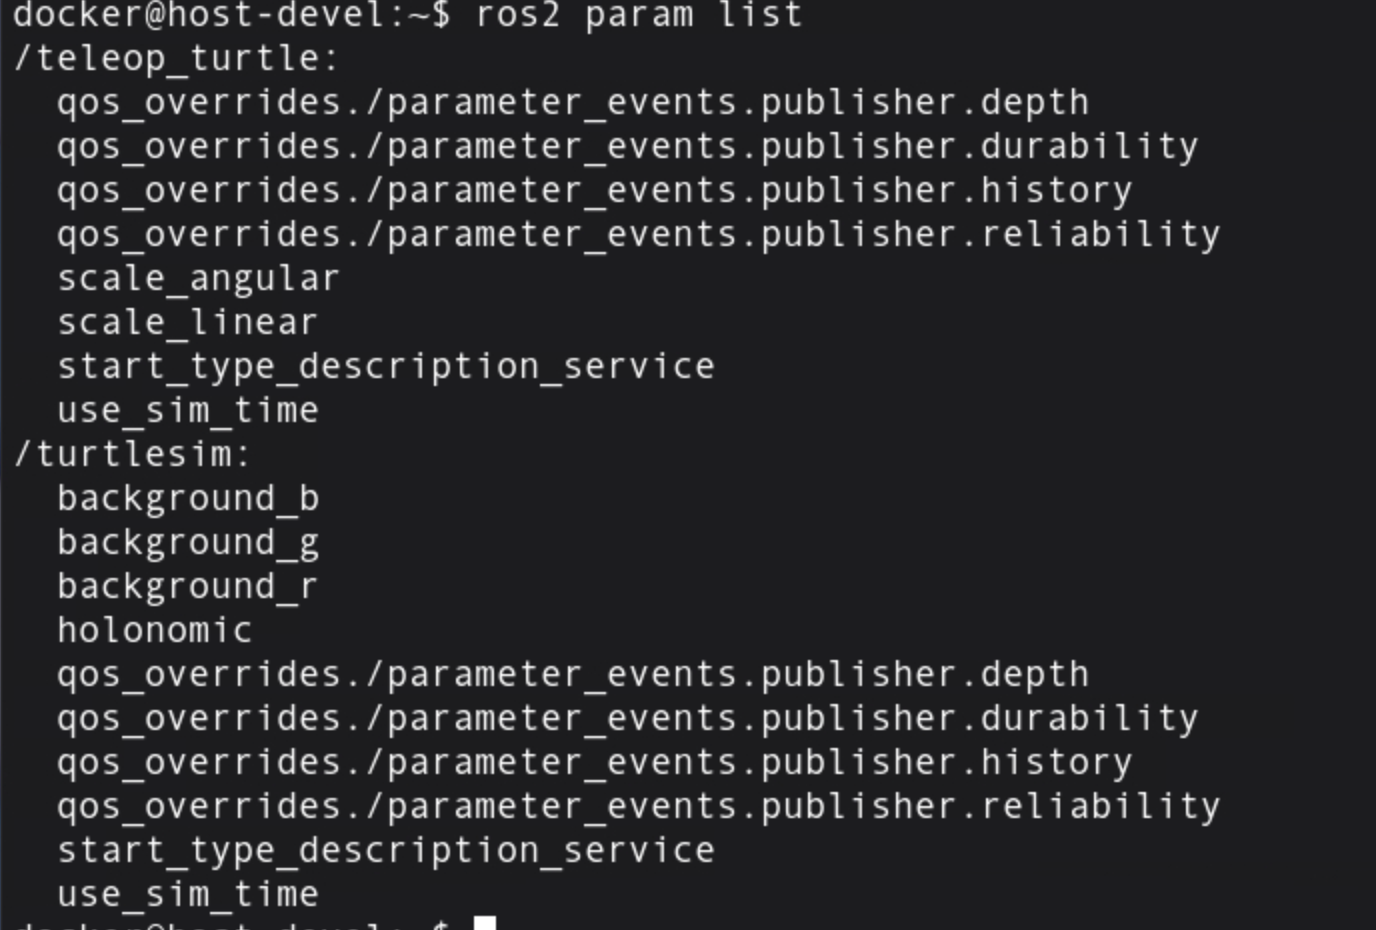
\includegraphics[width=0.75\textwidth]{p1.6-1}
\end{figure}

\item ros2 get param
To see the type and value of a node's parameter:
\begin{lstlisting}[language=bash]
ros2 get param /turtlesim backgount_g
\end{lstlisting}
\begin{figure}[h]
	\setlength{\leftskip}{2.4em}
	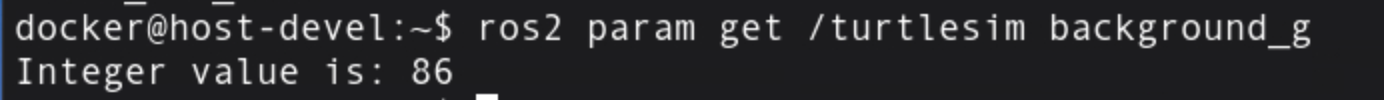
\includegraphics[width=0.94\textwidth]{p1.6-2}
\end{figure}

\newpage
\item ros2 set param\\
To set a parameter of a node:
\begin{lstlisting}[language=bash]
ros2 set param /turtlesim background_g 255
\end{lstlisting}
\begin{figure}[h]
	\setlength{\leftskip}{2.4em}
	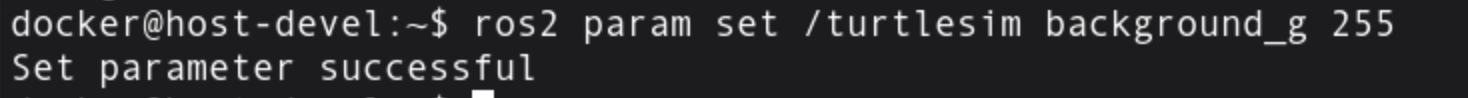
\includegraphics[width=0.94\textwidth]{p1.6-3}
\end{figure}
\begin{figure}[h]
	\centering
	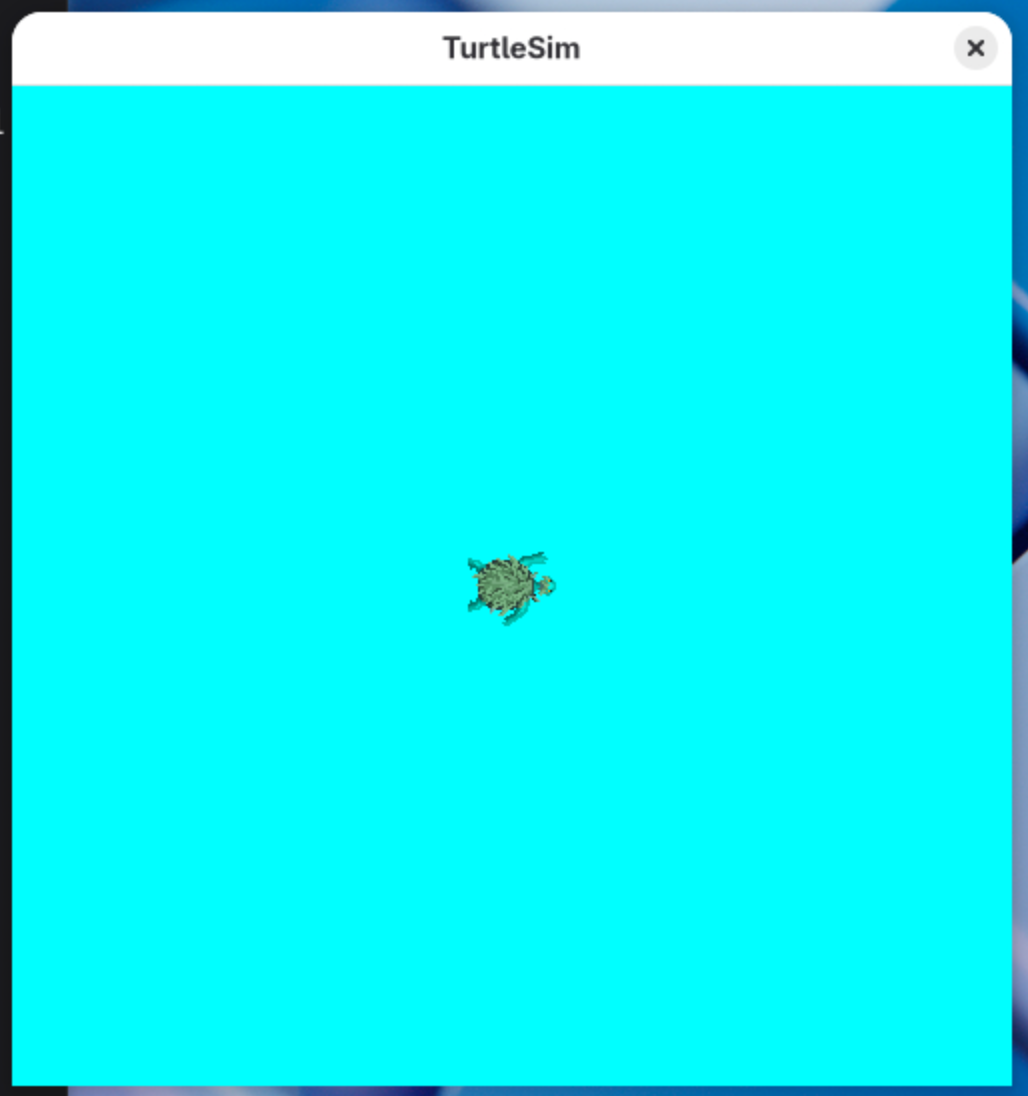
\includegraphics[width=0.4\textwidth]{p1.6-4}
\end{figure}

\item ros2 param dump\\
To see all parameters of a node:
\begin{lstlisting}[language=bash]
ros2 param dump /turtlesim
\end{lstlisting}
and it can also output to a file by appending \texttt{ > <filename>}.
\begin{figure}[h]
	\centering
	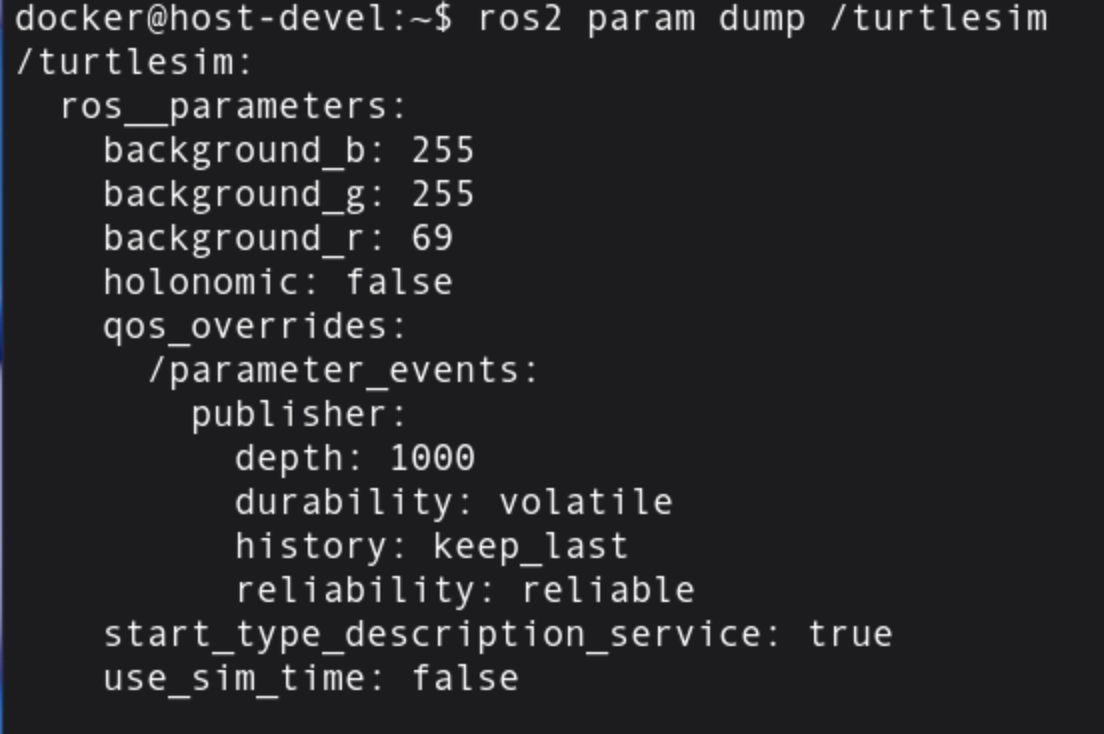
\includegraphics[width=0.75\textwidth]{p1.6-5}
\end{figure}

\newpage
\item ros2 param load\\
To load a file into a node:
\begin{lstlisting}[language=bash]
ros2 param load /turtlesim turtlesim.yaml
\end{lstlisting}
\begin{figure}[h]
	\centering
	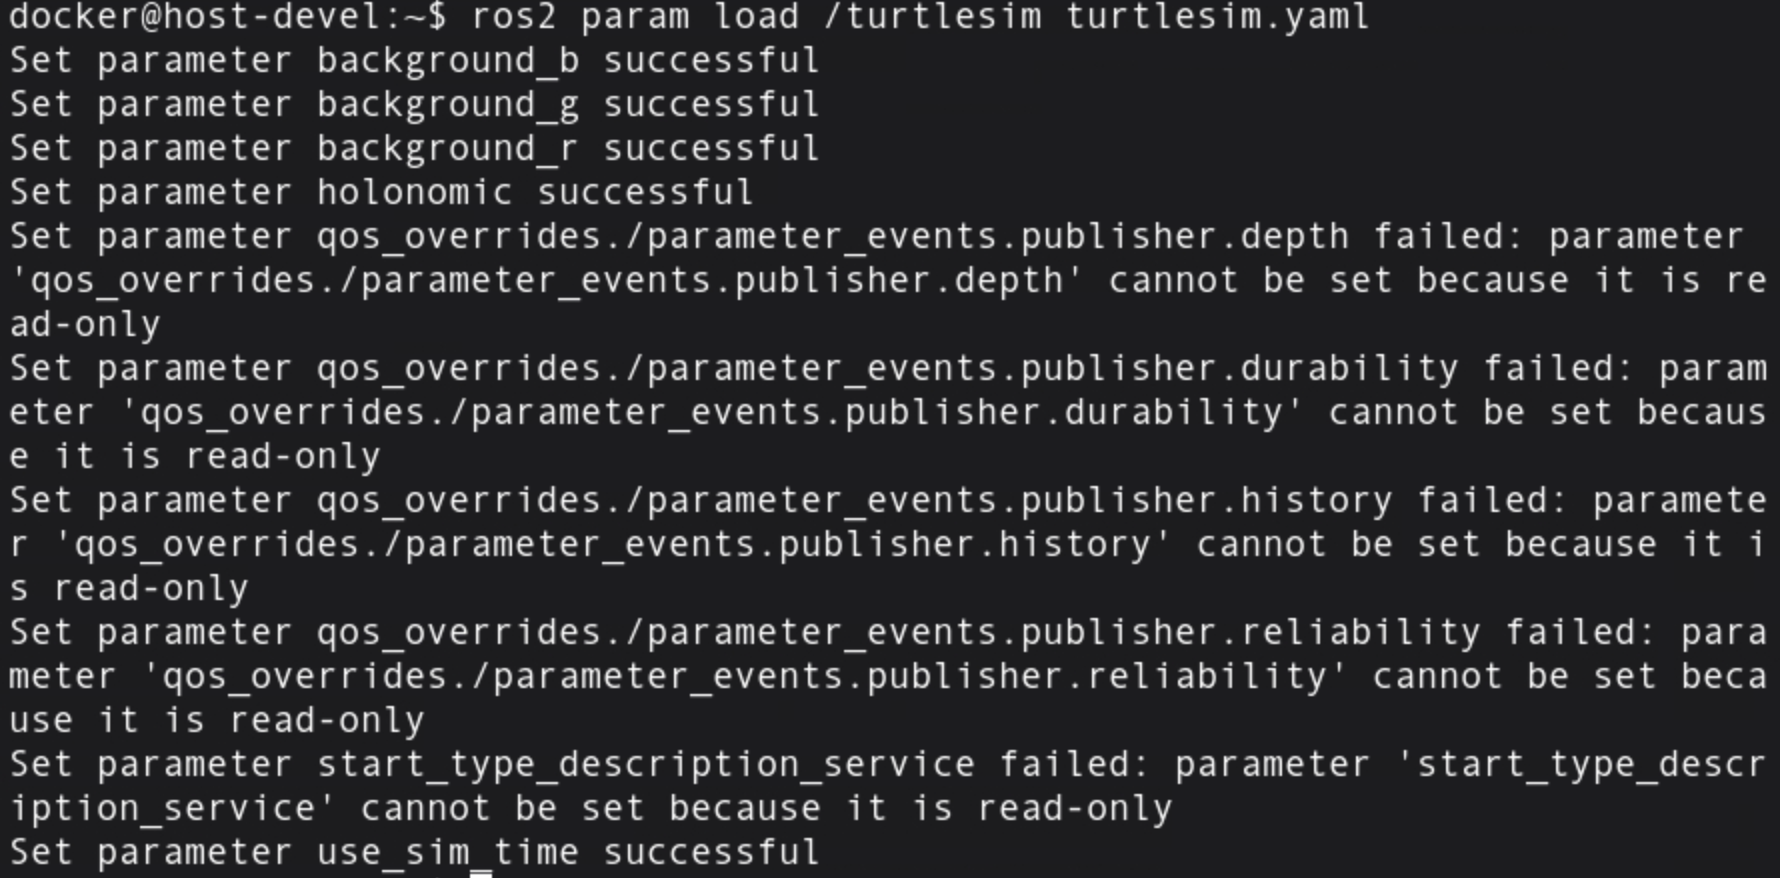
\includegraphics[width=0.75\textwidth]{p1.6-6}
\end{figure}
\item Load paramter file on node startup:\\
To load a parameter file to a new node:
\begin{lstlisting}[language=bash]
ros2 run turtlesim turtlesim_node --ros-args --params-file turtlesim.yaml
\end{lstlisting}
\begin{figure}[h]
	\setlength{\leftskip}{2.4em}
	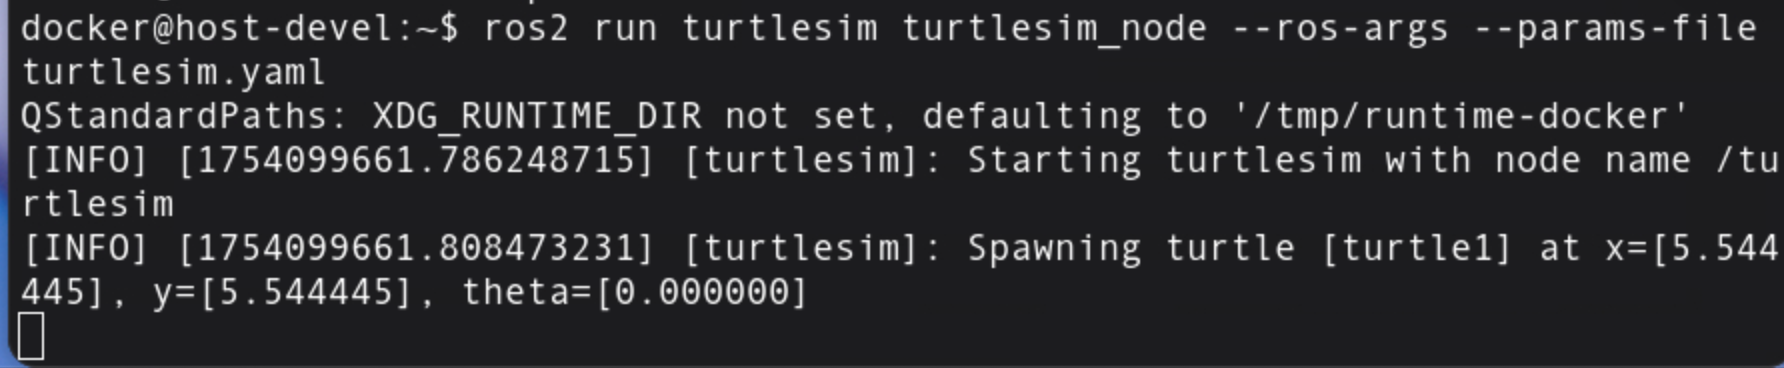
\includegraphics[width=0.94\textwidth]{p1.6-7}
\end{figure}
\end{enumerate}

\newpage
\subsection{Understanding actions}
\begin{enumerate}
	\item Setup
\begin{lstlisting}[language=bash]
ros2 run turtlesim turtlesim_node
ros2 run turtlesim turtle_teleop_key
\end{lstlisting}
\item Use actions\\
Use the operation in the \texttt{turtle\_teleop\_key}'s terminal, and observe the terminal of the node \texttt{turtlesim}:
\begin{figure}[h]
	\setlength{\leftskip}{2.4em}
	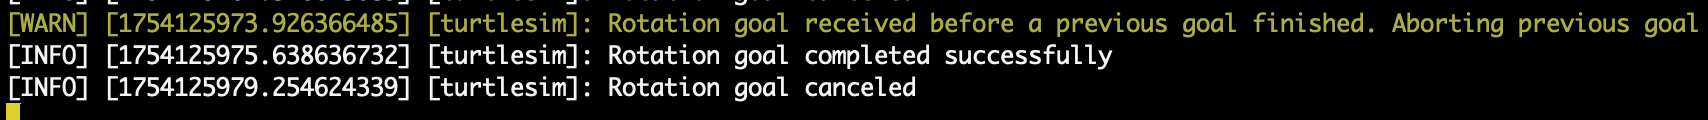
\includegraphics[width=0.94\textwidth]{p1.7-1}
\end{figure}
\item ros2 node info\\
To see the detail of a node:
\begin{lstlisting}[language=bash]
ros2 node info /turtlesim
\end{lstlisting}
\begin{figure}[h]
	\centering
	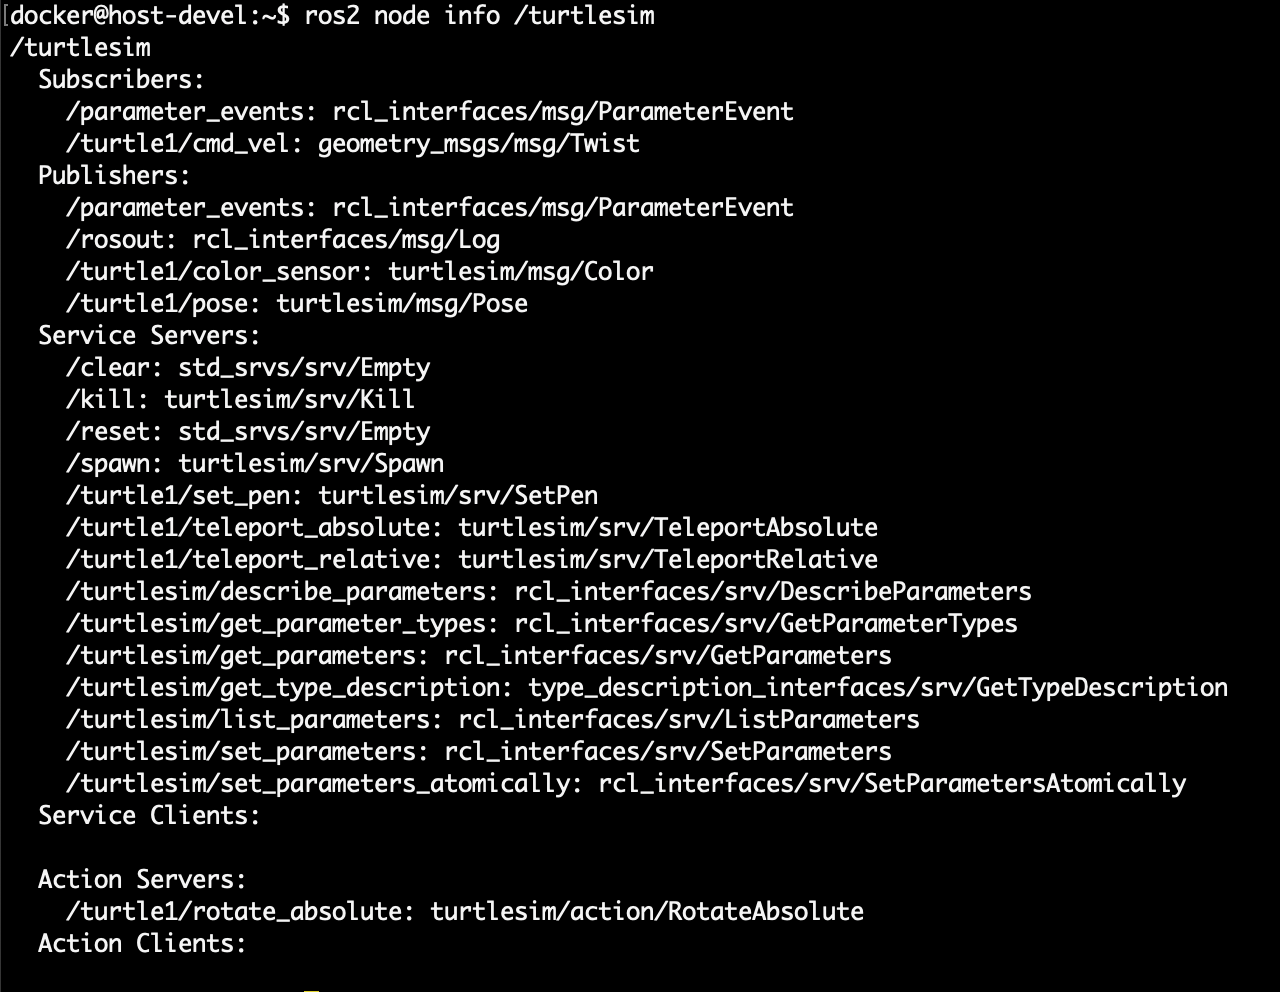
\includegraphics[width=0.75\textwidth]{p1.7-2}
\end{figure}
\item ros2 action list
To see all active actions:
\begin{lstlisting}[language=bash]
ros2 action list
\end{lstlisting}
Similarly, \texttt{-t} for type:
\begin{lstlisting}[language=bash]
ros2 action list -t
\end{lstlisting}
\begin{figure}[h]
	\setlength{\leftskip}{2.4em}
	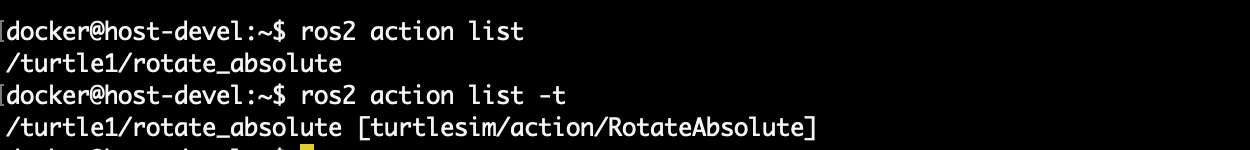
\includegraphics[width=0.94\textwidth]{p1.7-3}
\end{figure}

\item ros2 action info:
To see more detail about an action:
\begin{lstlisting}[language=bash]
ros2 action info /turtle1/rotate_absolute
\end{lstlisting}
\begin{figure}[h]
	\setlength{\leftskip}{2.4em}
	\includegraphics[width=0.94\textwidth]{p1.7-4}
\end{figure}

\item ros2 interface show:
To see the inerface of a type:
\begin{lstlisting}[language=bash]
ros2 interface show turtlesim/action/RotateAbsolute
\end{lstlisting}
\begin{figure}[h]
	\setlength{\leftskip}{2.4em}
	\includegraphics[width=0.94\textwidth]{p1.7-5}
\end{figure}

\item ros2 action send\_goal
To send an action goal from the command line directly:
\begin{lstlisting}[language=bash]
ros2 action send_goal /turtle1/rotate_absolute turtlesim/action/RotateAbsolute "{theta: 1.57}"
\end{lstlisting}
\begin{figure}[h]
	\setlength{\leftskip}{2.4em}
	\includegraphics[width=0.94\textwidth]{p1.7-6}
\end{figure}

\newpage
Add \texttt{--feedback} to see feedback:
\begin{figure}[h]
	\setlength{\leftskip}{2.4em}
	\includegraphics[width=0.94\textwidth]{p1.7-7}
\end{figure}
\end{enumerate}

\newpage
\subsection{Using \texttt{rqt\_console} to view logs}
\begin{enumerate}
	\item Setup
\begin{lstlisting}[language=bash]
ros2 run rqt_console rqt_console
\end{lstlisting}
\begin{figure}[h]
	\centering
	\includegraphics[width=0.4\textwidth]{p1.8-1}
\end{figure}

\item Messeages on rqt\_console\\
\begin{lstlisting}[language=bash]
ros2 topic pub -r 1 /turtle1/cmd_vel geometry_msgs/msg/Twist "{linear: {x: 2.0, y: 0.0, z: 0.0}, angular: {x: 0.0,y: 0.0,z: 0.0}}"
\end{lstlisting}
And we can see warning on the console:
\begin{figure}[h]
	\centering
	\includegraphics[width=0.75\textwidth]{p1.8-2}
\end{figure}

\newpage
We can use \texttt{--log-level} to set the logger level:
\begin{lstlisting}[language=bash]
ros2 run turtlesim turtlesim_node --ros-args --log-level WARN
\end{lstlisting}
And messages with level lower than \texttt{[WARN]}(\texttt{[INFO]}) cannot be seen.
\begin{figure}[h]
	\setlength{\leftskip}{2.4em}
	\includegraphics[width=0.94\textwidth]{p1.8-3}
\end{figure}
\end{enumerate}

\newpage
\subsection{Launching nodes}
\begin{itemize}
	\item Running a Luanch File
\begin{lstlisting}[language=bash]
ros2 launch turtlesim multisim.launch.py
\end{lstlisting}
We will see two turtlesim nodes:
\begin{figure}[h]
	\centering
	\includegraphics[width=0.8\textwidth]{p1.9-1}
\end{figure}
\end{itemize}

\newpage
\subsection{Recording and playing back data}
\begin{enumerate}
	\item Setup
\begin{lstlisting}[language=bash]
ros2 run turtlesim turtlesim_node
ros2 run turtlesim turtle_teleop_key
\end{lstlisting}
And also create a directory to store recordings.
\begin{lstlisting}[language=bash]
mkdir bag_files
\end{lstlisting}
\item Choose a topic
Use:
\begin{lstlisting}[language=bash]
ros2 topic list
\end{lstlisting}
We can choose a topic we want to record. Additionally, we can use the \texttt{topic echo} command to show the messages published to the topic.
\begin{lstlisting}[language=bash]
ros2 topic echo /turtle1/cmd_vel
\end{lstlisting}

\item ros2 bag record
\begin{enumerate}
	\item Record a single topic
\begin{lstlisting}[language=bash]
ros2 bag record /turtle1/cmd_vel
\end{lstlisting}
\begin{figure}[h]
	\setlength{\leftskip}{4.4em}
	\includegraphics[width=0.88\textwidth]{p1.10-1}
\end{figure}
\item Record multilple topics
\begin{lstlisting}[language=bash]
ros2 bag record <topic_1> <topic_2> ...
\end{lstlisting}
Option \texttt{-o} can name the file, and \texttt{-a} will record all topics.
\end{enumerate}

\newpage
\item ros2 bag info
\begin{lstlisting}[language=bash]
ros2 bag info <file_name>
\end{lstlisting}
\begin{figure}[h]
	\setlength{\leftskip}{2.4em}
	\includegraphics[width=0.94\textwidth]{p1.10-2}
\end{figure}

\item ros2 bag play
To play the recorded file (I reset the condition first):
\begin{lstlisting}[language=bash]
ros2 bag play <file_name>
\end{lstlisting}
\begin{figure}[h]
	\setlength{\leftskip}{2.4em}
	\includegraphics[width=0.94\textwidth]{p1.10-3}
\end{figure}
\end{enumerate}

\newpage
\section{Beginner: Client libraries (C++)}
\subsection{Using colcon to build packages}
\begin{enumerate}
	\item Prerequisites\\
Install colcon and ROS2
\item Create a workspace\\
Create a directory:
\begin{lstlisting}[language=bash]
mkdir -p ~/ros2_ws/src
cd ~/ros2_ws$
\end{lstlisting}
\item Add some sources
\begin{lstlisting}[language=bash]
git clone https://github.com/ros2/examples src/examples -b iron
\end{lstlisting}
\item Build the workspace
\begin{lstlisting}[language=bash]
colcon build --symlink-install
\end{lstlisting}
Run tests
\begin{lstlisting}[language=bash]
colcon test
\end{lstlisting}
\begin{figure}[h]
	\setlength{\leftskip}{2.4em}
	\includegraphics[width=0.94\textwidth]{2/p2.1-1}
\end{figure}
\item source the environment
\begin{lstlisting}[language=bash]
source install/setup.bash
\end{lstlisting}

\newpage
\item Try a demo
\begin{lstlisting}[language=bash]
ros2 run examples_rclcpp_minimal_subscriber subscriber_member_function
ros2 run examples_rclcpp_minimal_publisher publisher_member_function
\end{lstlisting}
\begin{figure}[h]
	\setlength{\leftskip}{2.4em}
	\includegraphics[width=0.94\textwidth]{2/p2.1-2}
	\includegraphics[width=0.94\textwidth]{2/p2.1-3}
\end{figure}

\item Setup \texttt{colcon\_cd}
\begin{lstlisting}[language=bash]
echo "source /usr/share/colcon_cd/function/colcon_cd.sh" >> ~/.bashrc
echo "export _colcon_cd_root=/opt/ros/iron/" >> ~/.bashrc
\end{lstlisting}
\end{enumerate}

\newpage
\subsection{Creating a workspace}
\begin{enumerate}
	\item Source ROS 2 environment\\
		Done in previous section.
	\item Create a new directory\\
		Done in previous section.
	\item Clone a sample repo\\
		In the \texttt{ros2\_ws/src} direcrtory:
\begin{lstlisting}[language=bash]
git clone https:/github.com/ros/ros_tutorials.git -b iron
\end{lstlisting}
	\item Resolve dependencies\\
		In \texttt{ros\_ws} directory:
\begin{lstlisting}[language=bash]
rosdep install -i --from-path src --rosdistro iron -y
\end{lstlisting}
\begin{figure}[h]
	\setlength{\leftskip}{2.4em}
	\includegraphics[width=0.94\textwidth]{2/p2.2-1}
\end{figure}
\item Build the workspace with colcon
\begin{lstlisting}[language=bash]
colcon build --parallel-workers 1
\end{lstlisting}
Using option \texttt{--parallel-workers 1} to prevent my memory run out of space.
\item source the overlay
\begin{lstlisting}[language=bash]
source install/local_setup.bash
\end{lstlisting}

\newpage
\item Modify the overlay\\
Find the file \texttt{turtle\_fram.cpp} in \\\texttt{~/ros2\_ws/src/ros\_tutorials/turtlesim/src}. Find the function \texttt{setWindowTitle()} and change the value.
\begin{lstlisting}[language=bash]
ros2 run turtlesim turtlesim_node
\end{lstlisting}
To see underlay, open a new terminal:
\begin{lstlisting}[language=bash]
ros2 run turtlesim turtlesim_node
\end{lstlisting}
\begin{figure}[h]
	\centering
	\includegraphics[width=0.75\textwidth]{2/p2.2-2}
\end{figure}
\end{enumerate}

\newpage
\subsection{Creating a package}
Before proceeding to this step, I went through the official CMake tutorial to make sure I understand the whole concept.
\begin{enumerate}
	\item Create a package\\
		In the directory \texttt{~/ros2\_ws/src}:
\begin{lstlisting}[language=bash]
ros2 pkg create --build-type ament_cmake --license Apache-2.0 --node-name my_node my_package
\end{lstlisting}
\begin{figure}[h]
	\centering
	\includegraphics[width=0.75\textwidth]{2/p2.3-1}
\end{figure}
\item Build a package
\begin{lstlisting}[language=bash]
colcon build --packages-select my_package
\end{lstlisting}
\begin{figure}[h]
	\setlength{\leftskip}{2.4em}
	\includegraphics[width=0.94\textwidth]{2/p2.3-2}
\end{figure}
\item Source the setup file
\begin{lstlisting}[language=bash]
source install/local_setup.bash
\end{lstlisting}

\item Use the package
\begin{lstlisting}[language=bash]
ros2 run my_package my_node
\end{lstlisting}
\begin{figure}[h]
	\setlength{\leftskip}{2.4em}
	\includegraphics[width=0.94\textwidth]{2/p2.3-3}
\end{figure}

\newpage
\item Examine package contents
	\begin{figure}[h]
		\centering
		\includegraphics[width=0.4\textwidth]{2/p2.3-4}
	\end{figure}
\item Customize \texttt{package.xml}
	\begin{figure}[h]
		\centering
		\includegraphics[width=0.8\textwidth]{2/p2.3-5}
	\end{figure}
\end{enumerate}

\newpage
\section{Writing a simple publisher and subscriber(C++)}
\begin{enumerate}
	\item Create a package
\begin{lstlisting}[language=bash]
ros2 pkg create --build-type ament_cmake --license Apache-2.0 cpp_pubsub
\end{lstlisting}
\begin{figure}[h]
	\centering
	\includegraphics[width=0.45\textwidth]{2/p2.4-1}
\end{figure}

\item Write the publisher node\\
Download the sample code:
\begin{lstlisting}[language=bash]
wget -O publisher_member_function.cpp https://raw.githubusercontent.com/ros2/examples/iron/rclcpp/topics/minimal_publisher/member_function.cpp
\end{lstlisting}
After download it, I spend some time to understand the code.
\end{enumerate}




\end{document}
